%! Author = Profesor
%! Date = 06/06/2024


\section{Ejercicios}

\subsection{Ejercicios}


\begin{exercise}
    En condiciones estándar, en la combustión de 1 g de etanol se desprenden 29,8 kJ y en la
    combustión de 1 g de ácido acético se liberan 14,5 kJ. Calcula: a) La entalpía de combustión estándar del etanol y la del ácido acético. b) La variación de entalpía estándar de la siguiente reacción: \ch{CH3CH2OH + O2 -> CH3COOH + H2O}. Datos: masas atómicas: M(C) = 12 u, M(O) = 16 u, M(H) = 1 u.

    \begin{solu}
%        \begin{figure}[H]
%            \centering
%            \includegraphics[scale=.5]{images/imagesUD4Termidonamica/UD4_Problemas/ejercicio_general_01.png}
%        \end{figure}
        a) Las masas molares son \(M(\ch{CH3CH2OH}) = 2(12)+6(1)+16 = \energia[j]{46}\,\ch{g/mol}\) y \(M(\ch{CH3COOH}) = 2(12)+4(1)+2(16) = \ch{60\ g/mol}\).

        La entalpía de combustión (por mol) se obtiene multiplicando el calor desprendido por gramo por la masa molar:
        \[
            \entalpia{comb, etanol} = -29{,}8 \; \ch{kJ/g} \times 46 \; \ch{g/mol} = \energia[kjmol]{-1370,8}
        \]
        \[
            \entalpia{comb, ácido acético} = -14{,}5 \; \ch{kJ/g} \times 60 \; \ch{g/mol} = \energia[kjmol]{-870}
        \]

        b) La reacción \(\ch{CH3CH2OH + O2 -> CH3COOH + H2O}\) se puede obtener combinando la combustión completa del etanol con la combustión completa (invertida) del ácido acético, mediante la ley de Hess:

        \begin{gather*}
            \ch{CH3CH2OH + 3 O2 -> 2 CO2 + 3 H2O} \qquad \entalpia{1} = \energia[kjmol]{-1370,8}\\
            \ch{2 CO2 + 2 H2O -> CH3COOH + 2 O2} \qquad -\entalpia{2} = \energia[kjmol]{+870}
        \end{gather*}

        Sumando ambas ecuaciones se cancelan \(2\;\ch{CO2}\), \(2\;\ch{O2}\) y \(2\;\ch{H2O}\), quedando la reacción pedida:
        \[
            \Delta H = \entalpia{1} - \entalpia{2} = -1370{,}8 - (-870) = \energia[kjmol]{-500,8}
        \]

        La reacción de oxidación del etanol a ácido acético es, por tanto, exotérmica, con \(\Delta H \approx \energia[kjmol]{-500,8}\).
    \end{solu}
\end{exercise}

\begin{exercise}
    Calcula: a) La variación de entalpía estándar para la descomposición de 1 mol de carbonato de calcio, en dióxido de carbono, y óxido de calcio. b) La energía necesaria para preparar 3 kg de óxido de calcio. Datos: M(Ca) = 40 u, M(O) = 16 u, \(\Delta H^0 \ch{CO2 \gas{}} = \energia[kjmol]{-393.5}\), \(\Delta H^0 \ch{CaCO3 \sld{}} = \energia[kjmol]{-1206}\), \(\Delta H^0 \ch{CaO \sld{}} = \energia[kjmol]{-635.6}\).

    \begin{solu}
%
%        \begin{figure}[H]
%            \centering
%            \includegraphics[scale=.5]{images/imagesUD4Termidonamica/UD4_Problemas/ejercicio_general_02.png}
%        \end{figure}

        a) La reacción de descomposición es \(\ch{CaCO3 (s) -> CaO (s) + CO2 (g)}\). Aplicando la ley de Hess:
        \[
            \Delta H^0 = \left[ \Delta H^0 (\ch{CaO}) + \Delta H^0 (\ch{CO2}) \right] - \Delta H^0 (\ch{CaCO3})
        \]
        \[
            \Delta H^0 = \left[ -635{,}6 + (-393{,}5) \right] - (-1206) = -1029{,}1 + 1206 = \energia[kjmol]{176,9}
        \]

        La descomposición del carbonato de calcio es, por tanto, endotérmica.

        b) La masa molar del óxido de calcio es \(M(\ch{CaO}) = 40+16 = \ch{56\ g/mol}\). Los moles de \ch{CaO} en 3 kg son:
        \[
            n(\ch{CaO}) = \frac{3000\ \ch{g}}{56\ \ch{g/mol}} = 53{,}57\ \text{mol}
        \]

        Como se forma 1 mol de \ch{CaO} por cada mol de \ch{CaCO3} descompuesto, con \(\Delta H^0 = \energia[kjmol]{176,9}\) por mol de \ch{CaO}:
        \[
            Q = 53{,}57\ \text{mol} \times \energia[kjmol]{176,9} = \energia[kj]{9476,8}
        \]

        Se necesitan, aproximadamente, \(\energia[kj]{9476,8}\) para preparar 3 kg de óxido de calcio.
    \end{solu}
\end{exercise}

\begin{exercise}
    Considera las siguientes reacciones químicas:

    I) \ch{A + B -> C}  \(\Delta H_1 = \energia[kj]{-145}\)

    II) \ch{3 A -> D + E}  \(\Delta H_2 = \energia[kj]{250}\)

    Dibuja un diagrama entálpico para cada una de las reacciones, justificando los dibujos.


    \begin{solu}

%        \begin{figure}[H]
%            \centering
%            \includegraphics[scale=.5]{images/imagesUD4Termidonamica/UD4_Problemas/ejercicio_general_03.png}
%        \end{figure}

        En un diagrama entálpico se representa la entalpía (energía) en el eje vertical, situando en un nivel horizontal a los reactivos y en otro nivel horizontal a los productos; una flecha vertical entre ambos niveles indica el sentido y el valor de \(\Delta H\).

        \textbf{Reacción I} (\(\ch{A + B -> C}\), \(\Delta H_1 = \energia[kj]{-145}\)): al ser \(\Delta H_1 < 0\), la reacción es \textbf{exotérmica}. Los reactivos (\(\ch{A+B}\)) se sitúan en un nivel de energía \textbf{superior} y el producto (C) en un nivel \textbf{inferior}, con una flecha descendente de \(A+B\) hacia \(C\) de magnitud \(\energia[kj]{145}\), que representa la energía liberada al entorno.

        \textbf{Reacción II} (\(\ch{3 A -> D + E}\), \(\Delta H_2 = \energia[kj]{250}\)): al ser \(\Delta H_2 > 0\), la reacción es \textbf{endotérmica}. Los reactivos (\(3\ch{A}\)) se sitúan en un nivel de energía \textbf{inferior} y los productos (\(\ch{D+E}\)) en un nivel \textbf{superior}, con una flecha ascendente de \(3A\) hacia \(D+E\) de magnitud \(\energia[kj]{250}\), que representa la energía absorbida del entorno.
    \end{solu}

\end{exercise}

\begin{exercise}
    Sabiendo que en la combustión de 1 kg de carbón se desprenden \energia[kj]{3.81e4}. Calcula:
    a) La entalpía estándar de combustión.
    b) La energía que se desprende en la combustión de 1 kg de \ch{CH4}.
    c) El volumen de \ch{CH4}, medido a 25 ºC y 1 atm de presión, que es necesario quemar para
    producir la misma energía que en la combustión de 1 kg de carbón.


    \begin{solu}

%        \begin{figure}[H]
%            \centering
%            \includegraphics[scale=.5]{images/imagesUD4Termidonamica/UD4_Problemas/ejercicio_general_04.png}
%        \end{figure}

        a) Suponiendo que el carbón es esencialmente carbono, \(M(\ch{C}) = \ch{12\ g/mol}\), en 1 kg hay:
        \[
            n(\ch{C}) = \frac{1000\ \ch{g}}{12\ \ch{g/mol}} = 83{,}33\ \text{mol}
        \]

        La entalpía estándar de combustión (por mol) es:
        \[
            \entalpia{comb} = \frac{-\energia[kj]{3,81e4}}{83{,}33\ \text{mol}} = \energia[kjmol]{-457,2}
        \]

        b) Tomando el valor tabulado de la entalpía de combustión del metano, \(\entalpia{comb, \ch{CH4}} = \energia[kjmol]{-890}\), y con \(M(\ch{CH4}) = \ch{16\ g/mol}\), en 1 kg hay:
        \[
            n(\ch{CH4}) = \frac{1000\ \ch{g}}{16\ \ch{g/mol}} = 62{,}5\ \text{mol}
        \]
        \[
            Q = 62{,}5\ \text{mol} \times \energia[kjmol]{890} = \energia[kj]{55625}
        \]

        c) Los moles de \ch{CH4} necesarios para desprender la misma energía que 1 kg de carbón (\(\energia[kj]{3,81e4}\)) son:
        \[
            n(\ch{CH4}) = \frac{\energia[kj]{3,81e4}}{\energia[kjmol]{890}} = 42{,}81\ \text{mol}
        \]

        Aplicando la ecuación de los gases ideales a 25 ºC (298 K) y 1 atm:
        \[
            V = \frac{nRT}{P} = \frac{42{,}81 \times 0{,}082 \times 298}{1} = \volumen[l]{1046}
        \]
    \end{solu}
\end{exercise}

\begin{exercise}
    La entalpía de combustión del benceno es \energia[kjmol]{-3267.4}. Calcula: a) El valor de la entalpía de formación del benceno líquido. b) La energía implicada en la combustión de 100 g
    de benceno líquido.


    \begin{solu}

%        \begin{figure}[H]
%            \centering
%            \includegraphics[scale=.5]{images/imagesUD4Termidonamica/UD4_Problemas/ejercicio_general_05.png}
%        \end{figure}

        a) La combustión del benceno líquido es \(\ch{C6H6 (l) + 15/2 O2 (g) -> 6 CO2 (g) + 3 H2O (l)}\). Usando \(\Delta H^0_f (\ch{CO2}) = \energia[kjmol]{-393,5}\) y \(\Delta H^0_f (\ch{H2O, l}) = \energia[kjmol]{-285,8}\):
        \[
            \Delta H^0_{comb} = \left[6\,\Delta H^0_f(\ch{CO2}) + 3\,\Delta H^0_f(\ch{H2O})\right] - \Delta H^0_f(\ch{C6H6})
        \]
        \[
            -3267{,}4 = \left[6(-393{,}5)+3(-285{,}8)\right] - \Delta H^0_f(\ch{C6H6}) = -3218{,}4 - \Delta H^0_f(\ch{C6H6})
        \]
        \[
            \Delta H^0_f(\ch{C6H6}) = -3218{,}4 + 3267{,}4 = \energia[kjmol]{49,0}
        \]

        b) La masa molar del benceno es \(M(\ch{C6H6}) = 6(12)+6(1) = \ch{78\ g/mol}\). Los moles en 100 g son:
        \[
            n = \frac{100\ \ch{g}}{78\ \ch{g/mol}} = 1{,}282\ \text{mol}
        \]
        \[
            Q = 1{,}282\ \text{mol} \times \energia[kjmol]{3267,4} = \energia[kj]{4189,1}
        \]

        Se liberan, aproximadamente, \(\energia[kj]{4189,1}\) en la combustión de 100 g de benceno.
    \end{solu}
\end{exercise}

\begin{exercise}
    Se almacena propano, \ch{C3H8}, en una cisterna para utilizarlo como combustible:
    a) Calcula su entalpía estándar de combustión.
    b) Calcula la energía que se desprenderá al quemar \volumen[metroscubicos]{1} de dicho combustible gaseoso
    medido en condiciones normales de presión y temperatura.


    \begin{solu}

%        \begin{figure}[H]
%            \centering
%            \includegraphics[scale=.5]{images/imagesUD4Termidonamica/UD4_Problemas/ejercicio_general_06.png}
%        \end{figure}

        a) La combustión del propano es \(\ch{C3H8 (g) + 5 O2 (g) -> 3 CO2 (g) + 4 H2O (l)}\). Con \(\Delta H^0_f (\ch{C3H8}) = \energia[kjmol]{-103,8}\), \(\Delta H^0_f (\ch{CO2}) = \energia[kjmol]{-393,1}\) y \(\Delta H^0_f (\ch{H2O, l}) = \energia[kjmol]{-285,8}\):
        \[
            \Delta H^0_{comb} = \left[3\,\Delta H^0_f(\ch{CO2}) + 4\,\Delta H^0_f(\ch{H2O})\right] - \Delta H^0_f(\ch{C3H8})
        \]
        \[
            \Delta H^0_{comb} = \left[3(-393{,}1)+4(-285{,}8)\right] - (-103{,}8) = -2322{,}5 + 103{,}8 = \energia[kjmol]{-2218,7}
        \]

        b) A condiciones normales (0 ºC = 273 K, 1 atm), en \volumen[metroscubicos]{1} = 1000 L de propano gaseoso hay:
        \[
            n = \frac{PV}{RT} = \frac{1 \times 1000}{0{,}082 \times 273} = 44{,}67\ \text{mol}
        \]
        \[
            Q = 44{,}67\ \text{mol} \times \energia[kjmol]{2218,7} = \energia[kj]{99111}
        \]

        Se desprenden, aproximadamente, \(\energia[kj]{99111}\) (unos \energia[kj]{9,91e4}) al quemar 1 \si{\cubic\metre} de propano en condiciones normales.
    \end{solu}
\end{exercise}
\begin{exercise}
    El sulfuro de zinc al tratarlo con oxígeno reacciona según:

    \begin{equation*}
        \ch{ZnS \sld{} + O2 \gas{} → ZnO \sld{} + SO2 \gas{}}
    \end{equation*}

    Si las entalpías de formación de las diferentes especies son:  \(\Delta H^0_f (\ch{ZnS}) = \energia[kjmol]{-184.1}\), \(\Delta H^0_f (\ch{ZnO}) = \energia[kjmol]{-349.3}\), \(\Delta H^0_f (\ch{SO2}) = \energia[kjmol]{-70.9}\)

    a) Ajusta la ecuación química.
    b) ¿Cuál será el calor, a presión constante de 1 atm, que se desprenderá cuando reacciones
    17 g de sulfuro de zinc en exceso de oxígeno?
    c) ¿Cuántos litros de SO2 medidos a 25 ºC y 1 atm se obtendrán?
    Datos: M(S) = 32 u, M(O) = 16 u,  \ctegases{}

    \begin{solu}

%        \begin{figure}[H]
%            \centering
%            \includegraphics[scale=.5]{images/imagesUD4Termidonamica/UD4_Problemas/ejercicio_general_07.png}
%        \end{figure}

        a) Ajustando la ecuación (Zn y S ya están ajustados; se ajusta el O contando 1 O en \ch{ZnO} y 2 en \ch{SO2}, total 3 O en productos, por lo que se necesitan 3/2 \ch{O2}; multiplicando por 2 para evitar fracciones):
        \[
            \ch{2 ZnS (s) + 3 O2 (g) -> 2 ZnO (s) + 2 SO2 (g)}
        \]

        b) La entalpía de esta reacción (para 2 mol de \ch{ZnS}) es:
        \[
            \Delta H^0 = \left[2\,\Delta H^0_f(\ch{ZnO}) + 2\,\Delta H^0_f(\ch{SO2})\right] - 2\,\Delta H^0_f(\ch{ZnS})
        \]
        \[
            \Delta H^0 = \left[2(-349{,}3)+2(-70{,}9)\right] - 2(-184{,}1) = -840{,}4+368{,}2 = \energia[kj]{-472,2}
        \]

        Por mol de \ch{ZnS}: \(\Delta H^0 = -472{,}2/2 = \energia[kjmol]{-236,1}\).

        Con \(M(\ch{ZnS}) = 65{,}4+32 = \ch{97,4\ g/mol}\) (tomando \(M(\ch{Zn}) = 65{,}4\ \ch{u}\)), los moles en 17 g son:
        \[
            n(\ch{ZnS}) = \frac{17\ \ch{g}}{97{,}4\ \ch{g/mol}} = 0{,}1745\ \text{mol}
        \]
        \[
            Q = 0{,}1745\ \text{mol} \times \energia[kjmol]{236,1} = \energia[kj]{41,2}
        \]

        Se desprenden, aproximadamente, \(\energia[kj]{41,2}\).

        c) Como la relación estequiométrica \ch{ZnS}:\ch{SO2} es 1:1, se forman también \(0{,}1745\) mol de \ch{SO2}. A 25 ºC (298 K) y 1 atm:
        \[
            V = \frac{nRT}{P} = \frac{0{,}1745 \times 0{,}082 \times 298}{1} = \volumen[l]{4,27}
        \]
    \end{solu}
\end{exercise}

\begin{exercise}
    a) Calcula la entalpía estándar de la reacción:

    \begin{equation*}
        \ch{CaC2 \sld{} + 2 H2O \lqd{} -> Ca (OH)2 \sld{} + C2H2 \lqd{}}
    \end{equation*}

    b) ¿Qué calor se desprende en la combustión de 100 dm3 de acetileno, medidos a 25 ºC y
    1 atm?
    Datos: \(\Delta H^0_f (\ch{CaC2}) = \energia[kjmol]{-59}\), \(\Delta H^0_f (\ch{C2H2}) = \energia[kjmol]{227}\), \(\Delta H^0_f (\ch{H2O}) = \energia[kjmol]{-285.8}\), \(\Delta H^0_f (\ch{Ca(OH)2}) = \energia[kjmol]{-986}\), \(\Delta H^0_f (\ch{CO2}) = \energia[kjmol]{-393.5}\).


    \begin{solu}

%        \begin{figure}[H]
%            \centering
%            \includegraphics[scale=.5]{images/imagesUD4Termidonamica/UD4_Problemas/ejercicio_general_08.png}
%            \includegraphics[scale=.5]{images/imagesUD4Termidonamica/UD4_Problemas/ejercicio_general_08b.png}
%        \end{figure}

        a) Aplicando la ley de Hess a la reacción \(\ch{CaC2 (s) + 2 H2O (l) -> Ca(OH)2 (s) + C2H2 (l)}\):
        \[
            \Delta H^0 = \left[\Delta H^0_f(\ch{Ca(OH)2}) + \Delta H^0_f(\ch{C2H2})\right] - \left[\Delta H^0_f(\ch{CaC2}) + 2\,\Delta H^0_f(\ch{H2O})\right]
        \]
        \[
            \Delta H^0 = \left[-986+227\right] - \left[-59+2(-285{,}8)\right] = -759 - (-630{,}6) = \energia[kjmol]{-128,4}
        \]

        b) La combustión del acetileno es \(\ch{C2H2 (g) + 5/2 O2 (g) -> 2 CO2 (g) + H2O (l)}\):
        \[
            \Delta H^0_{comb} = \left[2\,\Delta H^0_f(\ch{CO2}) + \Delta H^0_f(\ch{H2O})\right] - \Delta H^0_f(\ch{C2H2})
        \]
        \[
            \Delta H^0_{comb} = \left[2(-393{,}5)+(-285{,}8)\right] - 227 = -1072{,}8-227 = \energia[kjmol]{-1299,8}
        \]

        A 25 ºC (298 K) y 1 atm, los moles de acetileno en 100 \si{\deci\metre\cubed} = 100 L son:
        \[
            n = \frac{PV}{RT} = \frac{1 \times 100}{0{,}082 \times 298} = 4{,}092\ \text{mol}
        \]
        \[
            Q = 4{,}092\ \text{mol} \times \energia[kjmol]{1299,8} = \energia[kj]{5319,3}
        \]

        Se desprenden, aproximadamente, \(\energia[kj]{5319,3}\) en la combustión de 100 \si{\deci\metre\cubed} de acetileno.
    \end{solu}
\end{exercise}

\begin{exercise}
    Considera la reacción de combustión del butano gaseoso:
    a) Formula y ajusta dicha reacción.
    b) Estima la variación de entalpía de la reacción a partir de las energías de enlace.


    \begin{solu}

%        \begin{figure}[H]
%            \centering
%            \includegraphics[scale=.5]{images/imagesUD4Termidonamica/UD4_Problemas/ejercicio_general_09.png}
%        \end{figure}

        a) El butano es \(\ch{CH3-CH2-CH2-CH3}\) (\ch{C4H10}). Su combustión, ajustada (multiplicando por 2 para evitar fracciones), es:
        \[
            \ch{2 C4H10 (g) + 13 O2 (g) -> 8 CO2 (g) + 10 H2O (g)}
        \]

        b) El butano tiene, por molécula, 3 enlaces \ch{C-C} y 10 enlaces \ch{C-H}. Usando la tabla de entalpías de enlace (Figura \ref{fig:entalpias_de_enlace}): \(\ch{C-C}=\SI{347}{\kjpmol}\), \(\ch{C-H}=\SI{415}{\kjpmol}\), \(\ch{O=O}=\SI{494}{\kjpmol}\), \(\ch{C=O}=\SI{735}{\kjpmol}\), \(\ch{O-H}=\SI{460}{\kjpmol}\).

        Enlaces rotos (2 mol de butano + 13 mol de \ch{O2}):
        \[
            \sum \Delta H_{rotos} = 2\left[3(347)+10(415)\right] + 13(494) = 2(1041+4150)+6422 = 10382+6422 = \energia[kj]{16804}
        \]

        Enlaces formados (8 mol \ch{CO2}, con 2 \ch{C=O} cada una, y 10 mol \ch{H2O}, con 2 \ch{O-H} cada una):
        \[
            \sum \Delta H_{formados} = 16(735)+20(460) = 11760+9200 = \energia[kj]{20960}
        \]

        Para 2 mol de butano:
        \[
            \Delta H = 16804-20960 = \energia[kj]{-4156}
        \]

        Por mol de butano:
        \[
            \Delta H_{comb} = \frac{-4156}{2} = \energia[kjmol]{-2078}
        \]

        Este valor es una estimación (el método de las entalpías de enlace es aproximado, y además supone agua en estado gaseoso); el valor experimental real es más negativo.
    \end{solu}
\end{exercise}
\begin{exercise}
    Dadas las reacciones:
    \begin{gather*}
        a) \ch{KCl \sld{} -> K^+ \gas{} + Cl^- \gas{}} \Delta H = \energia[kj]{718}\\
        b) \ch{KCl \sld{} -> K \sld{} + 1/2 Cl2 \gas{}} \Delta H = \energia[kj]{436} \\
        c) \ch{K \sld{} + 1/2 Cl2 \gas{} -> K \gas{} + Cl \gas{}} \Delta H = \energia[kj]{211}
    \end{gather*}
    Calcula la \(\Delta H\) para la reacción

    \begin{equation*}
        \ch{K \gas{} + Cl \gas{} → K^+ \gas{} + Cl^- \gas{}}
    \end{equation*}


    \begin{solu}

%        \begin{figure}[H]
%            \centering
%            \includegraphics[scale=.5]{images/imagesUD4Termidonamica/UD4_Problemas/ejercicio_general_10.png}
%        \end{figure}

        Aplicando la ley de Hess, la reacción pedida, \(\ch{K (g) + Cl (g) -> K^+ (g) + Cl^- (g)}\), se obtiene combinando la reacción (c) invertida, la reacción (b) invertida y la reacción (a):

        \begin{gather*}
            \ch{K (g) + Cl (g) -> K (s) + 1/2 Cl2 (g)} \qquad -\Delta H_c = \energia[kj]{-211} \\
            \ch{K (s) + 1/2 Cl2 (g) -> KCl (s)} \qquad -\Delta H_b = \energia[kj]{-436} \\
            \ch{KCl (s) -> K^+ (g) + Cl^- (g)} \qquad \Delta H_a = \energia[kj]{718}
        \end{gather*}

        Sumando las tres ecuaciones se cancelan \ch{K(s)} y \ch{1/2 Cl2(g)} y \ch{KCl(s)}, quedando la reacción pedida:
        \[
            \Delta H = -\Delta H_c - \Delta H_b + \Delta H_a = -211-436+718 = \energia[kj]{71}
        \]

        La formación de los iones gaseosos \(\ch{K+}\) y \(\ch{Cl-}\) a partir de los átomos gaseosos K y Cl es, por tanto, endotérmica, con \(\Delta H = \energia[kj]{71}\) (coherente con que la energía de ionización del K es mayor, en valor absoluto, que la afinidad electrónica del Cl).
    \end{solu}
\end{exercise}
\begin{exercise}
    La entropía, \(S^0\), del etanol líquido es \energia[kjmol]{161}. Si la entalpía de vaporización del etanol es \energia[kjmol]{36.4}, a 25 ºC. ¿Cuál es el valor de la entropía absoluta, \(S^0\), del vapor de etanol en equilibrio con el líquido?


    \begin{solu}

%        \begin{figure}[H]
%            \centering
%            \includegraphics[scale=.5]{images/imagesUD4Termidonamica/UD4_Problemas/ejercicio_general_11.png}
%        \end{figure}

        Si el líquido y el vapor están en equilibrio a 25 ºC (298 K), la transición de fase es un proceso reversible en el que \(\Delta G_{vap} = 0\), por lo que:
        \[
            \Delta G_{vap} = \Delta H_{vap} - T \, \Delta S_{vap} = 0 \quad \Rightarrow \quad \Delta S_{vap} = \frac{\Delta H_{vap}}{T}
        \]
        \[
            \Delta S_{vap} = \frac{36{,}4 \; \text{kJ/mol}}{298\ \text{K}} = 0{,}1222\ \text{kJ/(mol·K)} = 122{,}2\ \text{J/(mol·K)}
        \]

        La entropía absoluta del vapor es la del líquido más el incremento de entropía en la vaporización:
        \[
            S^0_{vapor} = S^0_{líquido} + \Delta S_{vap} = 161 + 122{,}2 = \SI{283,2}{\joule\per\mole\per\kelvin}
        \]
    \end{solu}
\end{exercise}
\begin{exercise}
    Predice el signo de la entropía en las siguientes reacciones:
    \begin{gather*}
        a) \ch{2 NH3 \gas{} -> N2 \gas{} + 3 H2 \gas{}} \\
        b) \ch{C3H8 \gas{} + 5 O2 \gas{} -> 3 CO2 (g) + 4 H2O \lqd{}} \\
        c) \ch{2 KClO3 \sld{} -> 2 KCl \sld{} + 3 O2 \gas{}}
    \end{gather*}


    \begin{solu}

        La entropía es la magnitud termodinámica que da una medida del grado de desorden molecular
        de un sistema; por tanto, cuanto mayor sea el desorden interno de un sistema, mayor será su
        entropía.

        Las entropías de los gases son muy superiores a las de los líquidos y a su vez, las de los líquidos
        superan a las de los sólidos.

        En un sólido, los átomos están muy ordenados, su entropía es baja. En un líquido, los átomos
        pueden moverse, están más desordenados, su entropía es mayor. En un gas, los átomos están
        muy separados y se mueven rápidamente, el desorden y la entropía son máximas.

        a) \(\Delta S > 0\) En este caso, todas las sustancias son gaseosas. Al ser \(\Delta n = 4-2 > 0\), hay una variación positiva del número de moles de sustancias gaseosas (la cantidad de gas final es mayor
        que la cantidad de gas inicial) y el desorden ha aumentado.

        b) \(\Delta S < 0\) En este caso, la entropía de los productos de la ecuación (un gas y un líquido) es
        menor que la de los reactivos (dos gases).

        c) \(\Delta S > 0\)  En este caso, la entropía de los productos (un gas y un sólido) es mayor que la de
        los reactivos (un sólido).

    \end{solu}
\end{exercise}
\begin{exercise}
    Para la reacción de descomposición del peróxido de hidrógeno para dar agua y oxígeno a \temperatura[k]{298}. Calcula \(\Delta S^0\) estándar de la reacción. Datos: \(S^0 [\ch{H2O \lqd{}}] = \SI{69.9}{\joule\per\mole\per\kelvin}\), \(S^0 [\ch{H2O2 \lqd{}}] = \SI{109.6}{\joule\per\mole\per\kelvin}\), \(S^0 [\ch{O2 \gas{}}] = \SI{205.1}{\joule\per\mole\per\kelvin}\).


    \begin{solu}

%        \begin{figure}[H]
%            \centering
%            \includegraphics[scale=.5]{images/imagesUD4Termidonamica/UD4_Problemas/ejercicio_general_13.png}
%        \end{figure}

        La reacción de descomposición es \(\ch{2 H2O2 (l) -> 2 H2O (l) + O2 (g)}\). La variación de entropía estándar es:
        \[
            \Delta S^0 = \left[2\,S^0(\ch{H2O}) + S^0(\ch{O2})\right] - 2\,S^0(\ch{H2O2})
        \]
        \[
            \Delta S^0 = \left[2(69{,}9)+205{,}1\right] - 2(109{,}6) = 344{,}9-219{,}2 = \SI{125,7}{\joule\per\mole\per\kelvin}
        \]

        El valor positivo es coherente con el aumento de desorden al pasar de un líquido a una mezcla de líquido y gas (se genera 1 mol de gas, \ch{O2}, que no existía en los reactivos).
    \end{solu}
\end{exercise}

\begin{exercise}
    El acetileno o etino, \ch{C2H2}, se hidrogena para producir etano. Calcula a 298 K:

    a) La entalpía estándar de la reacción.
    b) La energía de Gibbs estándar de reacción.
    c) La entropía estándar de reacción.

    \datos{}: \(\Delta H^0_f (\ch{C2H2}) = \energia[kjmol]{227}\),  \(\Delta H^0_f (\ch{C2H6}) = \energia[kjmol]{-85}\), \(\Delta G^0_f (\ch{C2H2}) = \energia[kjmol]{209}\), \( \Delta G^0_f (\ch{C2H6}) = \energia[kjmol]{-33} \), \(S^0 [\ch{C2H2}] = \SI{200}{\joule\per\mole\per\kelvin}\), \(S^0 [\ch{C2H6}] = \SI{230}{\joule\per\mole\per\kelvin}\)


    \begin{solu}

%        \begin{figure}[H]
%            \centering
%            \includegraphics[scale=.5]{images/imagesUD4Termidonamica/UD4_Problemas/ejercicio_general_14.png}
%        \end{figure}

        La reacción de hidrogenación es \(\ch{C2H2 (g) + 2 H2 (g) -> C2H6 (g)}\).

        a) Entalpía estándar de reacción:
        \[
            \Delta H^0 = \Delta H^0_f(\ch{C2H6}) - \left[\Delta H^0_f(\ch{C2H2}) + 2\,\Delta H^0_f(\ch{H2})\right] = -85 - \left[227+0\right] = \energia[kjmol]{-312}
        \]

        b) Energía de Gibbs estándar de reacción:
        \[
            \Delta G^0 = \Delta G^0_f(\ch{C2H6}) - \left[\Delta G^0_f(\ch{C2H2}) + 2\,\Delta G^0_f(\ch{H2})\right] = -33 - \left[209+0\right] = \energia[kjmol]{-242}
        \]

        c) A partir de \(\Delta G^0 = \Delta H^0 - T\,\Delta S^0\), la entropía estándar de reacción es:
        \[
            \Delta S^0 = \frac{\Delta H^0 - \Delta G^0}{T} = \frac{-312-(-242)}{298}\ \text{kJ/(mol·K)} = \frac{-70}{298} = -0{,}2349\ \text{kJ/(mol·K)}
        \]
        \[
            \Delta S^0 = \SI{-234,9}{\joule\per\mole\per\kelvin}
        \]

        El valor negativo es coherente con la disminución del número de moles de gas (3 mol de gas en los reactivos frente a 1 mol de gas en los productos), lo que reduce el desorden del sistema.
    \end{solu}
\end{exercise}
\begin{exercise}
    Para la reacción:
    \begin{equation*}
        \ch{2 NO \gas{} + O2 \gas{} → 2 NO2 \gas{}}
    \end{equation*}

    Calcula: a) La entalpía de reacción a 25 ºC. b) Hasta qué temperatura la reacción será espontánea, sabiendo que para esta reacción \(S^0 = \SI{-146.4}{\joule\per\mole\per\kelvin}\). c) Si reaccionan 2 litros de \ch{NO}, medidos a 293 K y 1,2 atm con exceso de \ch{O2}. ¿Cuánto calor se desprende? \datos{}: \(\Delta H^0_f (\ch{NO \gas{}}) = \energia[kjmol]{90.25}\), \(\Delta H^0_f (\ch{NO2 \gas{}}) = \energia[kjmol]{227}\), \ctegases{}


    \begin{solu}

%        \begin{figure}[H]
%            \centering
%            \includegraphics[scale=.5]{images/imagesUD4Termidonamica/UD4_Problemas/ejercicio_general_14.png}
%        \end{figure}

        a) Entalpía de reacción a 25 ºC:
        \[
            \Delta H^0 = 2\,\Delta H^0_f(\ch{NO2}) - 2\,\Delta H^0_f(\ch{NO}) = 2(227) - 2(90{,}25) = 454-180{,}5 = \energia[kj]{273,5}
        \]

        b) Como \(\Delta H^0 = \energia[kj]{273,5} > 0\) y \(S^0 = \SI{-146,4}{\joule\per\mole\per\kelvin} < 0\), la energía de Gibbs
        \[
            \Delta G = \Delta H^0 - T\,\Delta S^0 = 273{,}5\ \text{kJ} - T \times (-0{,}1464\ \text{kJ/K}) = 273{,}5 + 0{,}1464\,T
        \]
        es siempre positiva para cualquier temperatura \(T>0\) (ambos sumandos son positivos), por lo que, con estos datos, \textbf{la reacción no es espontánea a ninguna temperatura} (no existe una temperatura de equilibrio real, ya que al igualar \(\Delta G=0\) se obtendría una temperatura negativa, sin sentido físico). Se trata del caso «\(\Delta H>0\), \(\Delta S<0\)», en el que el proceso directo nunca es favorable.

        c) A 293 K y 1,2 atm, los moles de \ch{NO} en 2 L son:
        \[
            n(\ch{NO}) = \frac{PV}{RT} = \frac{1{,}2 \times 2}{0{,}082 \times 293} = 0{,}0999\ \text{mol}
        \]

        Por cada 2 mol de \ch{NO} que reaccionan se intercambian \(\energia[kj]{273,5}\), es decir, \(136{,}75\) kJ/mol de \ch{NO}:
        \[
            Q = 0{,}0999\ \text{mol} \times \energia[kjmol]{136,75} = \energia[kj]{13,66}
        \]

        Según estos datos, el proceso absorbería (no desprendería) \(\energia[kj]{13,66}\), en coherencia con el carácter endotérmico obtenido en el apartado a).
    \end{solu}
\end{exercise}

\begin{exercise}
    Razona si son correctas o incorrectas las siguientes afirmaciones:

    \begin{enumerate}[label=\letraminuscula]
    \item En una reacción química no puede ser nunca \(\Delta G = 0\).
    \item \(\Delta G\) es independiente de la temperatura.
    \item La reacción no es espontánea si \(\Delta G > 0\).
    \item La reacción es muy rápida si \(\Delta G < 0\).
    \end{enumerate}


    \begin{solu}

        a) La afirmación «En una reacción química no puede ser nunca \(\Delta G = 0\) » es correcta. Cuando se
        alcanza un equilibrio químico, necesariamente ha de cumplirse que \(\Delta G = 0\), ya que se están
        verificando simultáneamente las reacciones directa e inversa con igual velocidad.

        b) La afirmación «\(\Delta G\) es independiente de la temperatura» es incorrecta. La variación de la energía libre de Gibbs vale: \(\Delta G = \Delta H - T\ \Delta S\), por lo que salvo que \(\Delta S = 0\), la variación de energía libre de Gibbs si depende de la temperatura.

        c) La afirmación «La reacción no es espontánea si \(\Delta G > 0\)» es correcta. Sabemos que si \(\Delta G < 0\) el proceso es espontáneo a la temperatura correspondiente, por tanto, si \(\Delta G > 0\), el proceso no
        será espontáneo a esa temperatura.

        d) La afirmación «La reacción es muy rápida si \(\Delta G < 0\)» es incorrecta. La magnitud energética
        relacionada con la velocidad de reacción es la energía de activación y no la energía libre de
        Gibbs. Un incremento en la energía de activación provoca una disminución de la velocidad de
        reacción

    \end{solu}
\end{exercise}
\begin{exercise}
    Calcula la entalpía de formación del etano a partir de la hidrogenación de eteno (reacción de eteno con hidrógeno). Las entalpías de enlace las tienes al final del documento.

    \begin{solu}

        La reacción de hidrogenación del eteno es:

        \begin{equation*}
            \ch{C2H4 \gas{} + H2 \gas{} -> C2H6 \gas{}}
        \end{equation*}

        A partir de las estructuras de Lewis, el eteno (\ch{CH2=CH2}) tiene 1 enlace \ch{C=C} y 4 enlaces \ch{C-H}; el hidrógeno tiene 1 enlace \ch{H-H}; y el etano (\ch{CH3-CH3}) tiene 1 enlace \ch{C-C} y 6 enlaces \ch{C-H}.

        Usando la tabla de entalpías de enlace (Figura \ref{fig:entalpias_de_enlace}): \(\ch{C=C} = \SI{610}{\kjpmol}\), \(\ch{C-H} = \SI{415}{\kjpmol}\), \(\ch{H-H} = \SI{436}{\kjpmol}\), \(\ch{C-C} = \SI{347}{\kjpmol}\).

        La variación de entalpía se calcula como la energía necesaria para romper los enlaces de los reactivos menos la energía liberada al formar los enlaces de los productos:

        \begin{equation*}
            \Delta H = \sum \Delta H_{enlaces \ rotos} - \sum \Delta H_{enlaces \ formados}
        \end{equation*}

        Enlaces rotos (reactivos): 1 \ch{C=C} + 4 \ch{C-H} (del eteno) + 1 \ch{H-H}:

        \begin{equation*}
            \sum \Delta H_{rotos} = 610 + 4(415) + 436 = 610 + 1660 + 436 = \energia[kjmol]{2706}
        \end{equation*}

        Enlaces formados (productos): 1 \ch{C-C} + 6 \ch{C-H} (del etano):

        \begin{equation*}
            \sum \Delta H_{formados} = 347 + 6(415) = 347 + 2490 = \energia[kjmol]{2837}
        \end{equation*}

        Por tanto:

        \begin{equation*}
            \Delta H = 2706 - 2837 = \energia[kjmol]{-131}
        \end{equation*}

        La hidrogenación del eteno para dar etano es exotérmica, con \(\Delta H \approx \energia[kjmol]{-131}\), un valor muy próximo al obtenido mediante entalpías de formación/combustión (\energia[kjmol]{-132}), lo que confirma la coherencia del método aproximado de las entalpías de enlace.

    \end{solu}
\end{exercise}

\begin{exercise}
    Calcula la entalpía de combustión del propano (\ch{C3H8}) a partir de los datos de entalpías de enlace que tienes al final del documento.

    \begin{solu}

        La reacción de combustión del propano, ajustada, es:

        \begin{equation*}
            \ch{C3H8 \gas{} + 5 O2 \gas{} -> 3 CO2 \gas{} + 4 H2O \gas{}}
        \end{equation*}

        El propano (\ch{CH3-CH2-CH3}) tiene 2 enlaces \ch{C-C} y 8 enlaces \ch{C-H}. Con la tabla de entalpías de enlace (Figura \ref{fig:entalpias_de_enlace}): \(\ch{C-C} = \SI{347}{\kjpmol}\), \(\ch{C-H} = \SI{415}{\kjpmol}\), \(\ch{O=O} = \SI{494}{\kjpmol}\), \(\ch{C=O} = \SI{735}{\kjpmol}\) (en el \ch{CO2}), \(\ch{O-H} = \SI{460}{\kjpmol}\).

        Enlaces rotos (reactivos): 2 \ch{C-C}, 8 \ch{C-H} (del propano) y 5 \ch{O=O} (del oxígeno):

        \begin{equation*}
            \sum \Delta H_{rotos} = 2(347) + 8(415) + 5(494) = 694 + 3320 + 2470 = \energia[kjmol]{6484}
        \end{equation*}

        Enlaces formados (productos): cada \ch{CO2} tiene 2 enlaces \ch{C=O} (3 mol de \ch{CO2} → 6 enlaces \ch{C=O}) y cada \ch{H2O} tiene 2 enlaces \ch{O-H} (4 mol de \ch{H2O} → 8 enlaces \ch{O-H}):

        \begin{equation*}
            \sum \Delta H_{formados} = 6(735) + 8(460) = 4410 + 3680 = \energia[kjmol]{8090}
        \end{equation*}

        Por tanto:

        \begin{equation*}
            \Delta H_{comb} = \sum \Delta H_{rotos} - \sum \Delta H_{formados} = 6484 - 8090 = \energia[kjmol]{-1606}
        \end{equation*}

        La combustión del propano es, como cabía esperar, muy exotérmica (\(\Delta H_{comb} \approx \energia[kjmol]{-1606}\)). El valor difiere del obtenido experimentalmente con datos de formación (en torno a \energia[kjmol]{-2220}, con agua líquida) porque el método de las entalpías de enlace es una aproximación que supone todas las especies en estado gaseoso, sin tener en cuenta la entalpía de condensación del agua ni las particularidades estructurales de cada compuesto.

    \end{solu}
\end{exercise}

\subsection{Cuestiones}


\begin{question}
    Establece las diferencias existentes entre una transformación isócora, isobara, una isoterma y una adiabática.


    \begin{solu}

%        \begin{figure}[H]
%            \centering
%            \includegraphics[scale=.3]{images/imagesUD4Termidonamica/UD4_Problemas/cuestion_01.png}
%        \end{figure}

        \begin{itemize}
            \item \textbf{Transformación isócora} (a volumen constante, \(V = \text{cte}\)): el sistema no realiza trabajo de expansión/compresión (\(W=0\)), por lo que todo el calor intercambiado se invierte en variar la energía interna: \(\Delta U = Q_v\).
            \item \textbf{Transformación isobara} (a presión constante, \(P = \text{cte}\)): el sistema puede realizar o recibir trabajo de expansión, \(W = P\,\Delta V\); el calor intercambiado a presión constante coincide con la variación de entalpía: \(Q_p = \Delta H\).
            \item \textbf{Transformación isoterma} (a temperatura constante, \(T = \text{cte}\)): para un gas ideal, la energía interna solo depende de la temperatura, por lo que \(\Delta U = 0\) y, por el primer principio, \(Q = W\) (todo el calor absorbido se transforma en trabajo, o viceversa).
            \item \textbf{Transformación adiabática} (sin intercambio de calor con el entorno, \(Q = 0\)): toda la variación de energía interna se debe al trabajo realizado: \(\Delta U = -W\).
        \end{itemize}
    \end{solu}
\end{question}

\begin{question}
    En un proceso, un sistema recibe 500 J de calor y realiza un trabajo de expansión de 280 J.
    ¿Qué cambio experimenta su energía interna?


    \begin{solu}

%        \begin{figure}[H]
%            \centering
%            \includegraphics[scale=.5]{images/imagesUD4Termidonamica/UD4_Problemas/cuestion_02.png}
%        \end{figure}

        Según el primer principio de la termodinámica, \(\Delta U = Q - W\), donde \(Q\) es el calor recibido por el sistema y \(W\) el trabajo realizado por el sistema. Con \(Q = \energia[j]{500}\) (recibido, positivo) y \(W = \energia[j]{280}\) (trabajo de expansión realizado por el sistema, positivo):
        \[
            \Delta U = Q - W = 500 - 280 = \energia[j]{220}
        \]

        La energía interna del sistema \textbf{aumenta} en \(\energia[j]{220}\).
    \end{solu}
\end{question}

\begin{question}
    Al quemarse la gasolina en un cilindro del motor de un coche se liberan 135 kJ. Si el trabajo
    realizado por los gases producidos en la combustión es de 54 kJ, calcula cuánto valdrá la
    variación de energía interna del sistema.


    \begin{solu}
%        \begin{figure}[H]
%            \centering
%            \includegraphics[scale=.5]{images/imagesUD4Termidonamica/UD4_Problemas/cuestion_03.png}
%        \end{figure}
        El sistema (los gases de combustión) libera calor al entorno, por lo que \(Q = \energia[kj]{-135}\), y realiza trabajo de expansión sobre el entorno, \(W = \energia[kj]{54}\). Aplicando el primer principio, \(\Delta U = Q - W\):
        \[
            \Delta U = -135 - 54 = \energia[kj]{-189}
        \]

        La energía interna del sistema \textbf{disminuye} en \(\energia[kj]{189}\).
    \end{solu}
\end{question}

\begin{question}
    ¿Por qué es necesario indicar en las ecuaciones termoquímicas el estado de agregación de
    las sustancias que intervienen en la reacción?


    \begin{solu}
        Porque el estado de agregación de los reactivos y de los productos, incluso las distintas formas
        cristalinas de un compuesto o las modificaciones alotrópicas de un elemento, junto con la temperatura y la presión, influyen en los valores de los calores de reacción
    \end{solu}
\end{question}

\subsection{Ejercicios PAU}

\begin{exerciseEVAU}
Las entalpías estándar de formación del butano gas \ch{C4H10}, dióxido de carbono gas \ch{CO2} y del agua líquida H2O son \num{-124,7}, \num{-393,5} y \num{-285,8} \unit{kjpmol}, respectivamente.
\begin{enumerate}[label=\letraminuscula]
    \item Escriba las reacciones ajustadas correspondientes a los procesos anteriores, así como la
correspondiente a la combustión del butano.
    \item Calcule la entalpía de combustión del butano en esas condiciones.
    \item Calcule a partir de los datos siguientes la variación de entropía de la reacción, su variación
de energía libre y determine si el proceso será espontáneo a la temperatura de 298 K.
\end{enumerate}
\textbf{Datos:}
% [FIGURA ORIGINAL] \includegraphics[scale=0.5]{images/imagesUD4Termidonamica/UD4_Problemas/pau_2023_julio_datos}
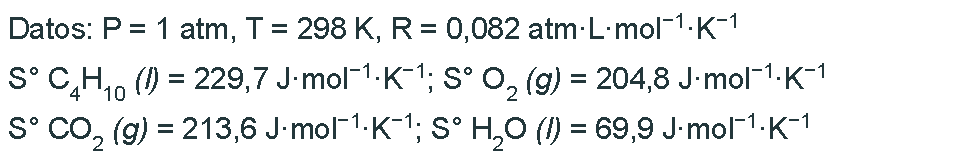
\includegraphics[width=0.75\linewidth]{FigurasSVG/UD4_Termodinamica/pdf/UD4_E01_datos_pau_2023_julio.pdf}
\begin{solu}

\end{solu}
\end{exerciseEVAU}

\begin{exerciseEVAU}
    Dada ls ecuación de la reacción de combustión del etanol:
    \begin{equation*}
        \ch{C2H6 \lqd{} + O2 \gas{} -> CO2 \gas{} + H2O \lqd{}}
    \end{equation*}
    \begin{enumerate}[label=\letraminuscula]
        \item Ajuste la ecuación y calcula la entalpía de combustión del etanol.
        \item Calcule la variación de entropía de esta reacción.
        \item Determine si el proceso será espontáneo a 25 ºC
    \end{enumerate}
    \textbf{Datos:}
    % [FIGURA ORIGINAL] \includegraphics[scale=0.5]{images/imagesUD4Termidonamica/UD4_Problemas/pau_2023_datos}
    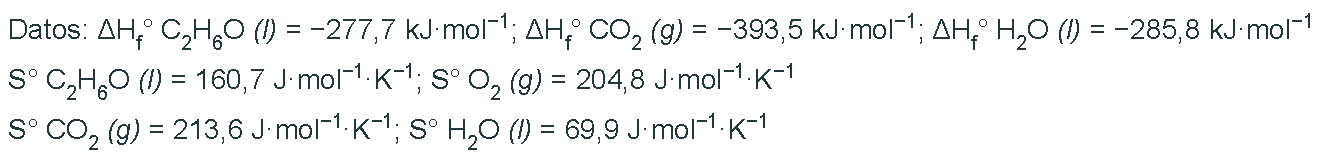
\includegraphics[width=0.95\linewidth]{FigurasSVG/UD4_Termodinamica/pdf/UD4_E02_datos_pau_2023.pdf}
\begin{solu}

\end{solu}
\end{exerciseEVAU}

\begin{exerciseEVAU}
    El aluminio es un agente eficiente para la reducción de óxidos metálicos. Un ejemplo de ello es la reducción
    del óxido de hierro (III), \ch{Fe2O3}, a hierro metálico según la siguiente reacción.
    \begin{centeredequation}
        \ch{Fe2O3 \sld{} + 2 Al \sld{} -> Al2O3 \sld{} + 2 Fe \sld{}}
    \end{centeredequation}
    \begin{enumerate}[label=\letraminuscula]
        \item Calcule la variación de entalpía estándar de esta reacción.
        \item Calcule el calor desprendido en la reducción de 100 g de \ch{Fe2O3}.
        \item Calcule la variación de energía libre de Gibbs a 298 K. ¿Es espontánea la reacción a esa
        temperatura? Justifique la respuesta.
    \end{enumerate}
    \textbf{Datos:} \(  \Delta H^{0}_{f}  [\ch{Fe2O3 \sld{}}] = \qty{- 821,37}{\kjpmol}; \Delta H^{0}_{f}  [\ch{Al2O3 \sld{}}] = \qty{- 1668,24}{\kjpmol};
%    S^0 [\ch{Fe2O3 \sld{}}]= \qty{90}{\jpmol}; S^{0} [\ch{Al2O3 \sld{}}] = \qty{51}{\jpmol}; S^0 [\ch{Al \sld{}}]= \qty{28,3}{\jpmol}; S^{0} [\ch{Fe \sld{}}]= \qty{27,2}{\jpmol}
    \)

    \begin{solu}

        \textbf{a) Entalpía estándar de la reacción}

        La reacción ya está ajustada:
        \begin{equation*}
            \ch{Fe2O3 \sld{} + 2 Al \sld{} -> Al2O3 \sld{} + 2 Fe \sld{}}
        \end{equation*}

        Aplicando la ley de Hess, la entalpía de reacción se calcula como la diferencia entre las entalpías de formación de productos y reactivos (recordando que la entalpía de formación de un elemento en su forma más estable, como \ch{Al \sld{}} y \ch{Fe \sld{}}, es cero):

        \begin{equation*}
            \Delta H^0_{rxn} = \left[ \Delta H^0_f (\ch{Al2O3}) + 2\, \Delta H^0_f (\ch{Fe}) \right] - \left[ \Delta H^0_f (\ch{Fe2O3}) + 2\, \Delta H^0_f (\ch{Al}) \right]
        \end{equation*}

        \begin{equation*}
            \Delta H^0_{rxn} = \left[ -1668,24 + 0 \right] - \left[ -821,37 + 0 \right] = \energia[kj]{-846.87}
        \end{equation*}

        Como \(\Delta H^0 < 0\), la reacción es exotérmica.

        \textbf{b) Calor desprendido en la reducción de 100 g de \ch{Fe2O3}}

        Calculamos la masa molar del \ch{Fe2O3} (M(Fe) = 55,85 u, M(O) = 16 u):

        \begin{equation*}
            M(\ch{Fe2O3}) = 2(55,85) + 3(16) = \SI{159.7}{\gram\per\mole}
        \end{equation*}

        Los moles de \ch{Fe2O3} que reaccionan son:

        \begin{equation*}
            n(\ch{Fe2O3}) = \dfrac{100 \ \si{\gram}}{159,7 \ \si{\gram\per\mole}} = 0,626 \ \text{mol}
        \end{equation*}

        Como la reacción libera \(846,87\) kJ por cada mol de \ch{Fe2O3} que reacciona:

        \begin{equation*}
            q = 0,626 \ \text{mol} \times \energia[kjmol]{846.87} = \energia[kj]{530.3}
        \end{equation*}

        Se desprenden, por tanto, \energia[kj]{530.3} en la reducción de 100 g de \ch{Fe2O3}.

        \textbf{c) Energía de Gibbs a 298 K y espontaneidad}

        En esta reacción todas las especies (reactivos y productos) son sólidos, por lo que no hay una variación significativa en el grado de desorden del sistema: el número de partículas gaseosas no cambia (de hecho no hay ninguna especie gaseosa), así que \(\Delta S^0 \approx 0\).

        En estas condiciones:

        \begin{equation*}
            \Delta G^0 = \Delta H^0 - T \Delta S^0 \approx \Delta H^0 = \energia[kj]{-846.87}
        \end{equation*}

        Como \(\Delta G^0 < 0\), la reacción \textbf{es espontánea} a 298 K. Esto es coherente con el hecho de que el aluminio es, en la práctica, un potente reductor de óxidos metálicos (proceso conocido como aluminotermia).

    \end{solu}
\end{exerciseEVAU}

\begin{exerciseEVAU}
    Existen bacterias que degradan la glucosa (\ch{C6H12O6}) mediante un proceso denominado fermentación
    alcohólica, en el cual se produce etanol (\ch{CH3-CH2OH}) y dióxido de carbono (\ch{CO2}) según la siguiente
    reacción:
    \begin{centeredequation}
        \ch{C6H12O6 \gas{} -> 2 CH3-CH3OH \lqd{} + 2 CO2 \gas{}}
    \end{centeredequation}
    \begin{enumerate}[label=\letraminuscula]
    \item Utilizando la Ley de Hess, determine la energía intercambiada en la fermentación de un mol
    de glucosa.
    \item Indique si dicha reacción es endotérmica o exotérmica, justificando la respuesta.
    \item Calcule la cantidad de calor que se produce en la fermentación de 1 Kg de glucosa.
    \end{enumerate}
    \textbf{Datos:}  Las entalpías de combustión de la glucosa y del etanol son –2815 kJ/mol y –1372 kJ/mol,
    respectivamente. Masas atómicas: (C) = 12 u; (O) = 16 u; (H) = 1 u.

    \begin{solu}

        \textbf{a) Energía intercambiada en la fermentación de un mol de glucosa (Ley de Hess)}

        La reacción de fermentación es:

        \begin{equation*}
            \ch{C6H12O6 \sld{} -> 2 CH3CH2OH \lqd{} + 2 CO2 \gas{}}
        \end{equation*}

        Para aplicar la ley de Hess necesitamos las reacciones de combustión de la glucosa y del etanol:

        \begin{align*}
            \text{(1)} \quad & \ch{C6H12O6 \sld{} + 6 O2 \gas{} -> 6 CO2 \gas{} + 6 H2O \lqd{}} \quad \Delta H_1 = \energia[kjmol]{-2815} \\
            \text{(2)} \quad & \ch{CH3CH2OH \lqd{} + 3 O2 \gas{} -> 2 CO2 \gas{} + 3 H2O \lqd{}} \quad \Delta H_2 = \energia[kjmol]{-1372}
        \end{align*}

        Para obtener la reacción de fermentación a partir de estas dos, mantenemos la reacción (1) y restamos dos veces la reacción (2) (es decir, invertimos dos veces la combustión del etanol y la sumamos a la de la glucosa):

        \begin{equation*}
            \Delta H_{ferm} = \Delta H_1 - 2 \Delta H_2 = -2815 - 2(-1372) = -2815 + 2744 = \energia[kjmol]{-71}
        \end{equation*}

        Por tanto, en la fermentación de 1 mol de glucosa se desprenden \energia[kjmol]{71}.

        \textbf{b) Carácter endotérmico o exotérmico}

        Como \(\Delta H_{ferm} = \energia[kjmol]{-71} < 0\), el proceso desprende calor al entorno, por lo que la reacción es \textbf{exotérmica}.

        \textbf{c) Calor producido en la fermentación de 1 kg de glucosa}

        La masa molar de la glucosa (\ch{C6H12O6}) es:

        \begin{equation*}
            M(\ch{C6H12O6}) = 6(12) + 12(1) + 6(16) = \SI{180}{\gram\per\mole}
        \end{equation*}

        Los moles contenidos en 1 kg (1000 g) de glucosa son:

        \begin{equation*}
            n = \dfrac{1000 \ \si{\gram}}{180 \ \si{\gram\per\mole}} = 5,56 \ \text{mol}
        \end{equation*}

        El calor desprendido será:

        \begin{equation*}
            q = 5,56 \ \text{mol} \times \energia[kjmol]{71} = \energia[kj]{394.4}
        \end{equation*}

        Se desprenden, por tanto, aproximadamente \energia[kj]{394.4} en la fermentación de 1 kg de glucosa.

    \end{solu}
\end{exerciseEVAU}


\begin{exerciseEVAU}
    \textbf{2024}.
    \begin{reaction*}
        C2H6O \lqd{} + O2 \gas{} -> CO2 \gas{} + H2O \lqd{}
    \end{reaction*}

    \begin{enumerate}[label=\letraminuscula]
         \item Ajuste la ecuación y calcule la entalpía de combustión del etanol.
         \item Calcule la variación de entropía de esta reacción.
         \item Determine si este proceso será espontáneo a \SI{25}{\celsius}.
    \end{enumerate}

    \datos{}: \( \Delta H^0_f\  \ch{C2H6O \lqd{}} = \SI{-277.7}{\kjpmol}  \); \( \Delta H^0_f\ \ch{CO2 \gas{}} = \SI{-393.5}{\kjpmol} \); \( \Delta H^0_f\ \ch{H2O \lqd{}} = \SI{-285.8}{\kjpmol} \); \( \Delta S^0_f\ \ch{C2H6O \lqd{}} = \SI{160.7}{\jpmolpk} \); \( \Delta S^0_f\ \ch{O2 \gas{}} = \SI{204.8}{\jpmolpk} \); \( \Delta S^0_f\ \ch{CO2 \gas{}} = \SI{213.6}{\jpmolpk} \); \( \Delta S^0_f\ \ch{H2O \lqd{}} = \SI{69.9}{\jpmolpk} \)
    \begin{solu}

        \textbf{a) Ajuste de la ecuación y entalpía de combustión del etanol}

        La ecuación ajustada de la combustión del etanol es:

        \begin{equation*}
            \ch{C2H6O \lqd{} + 3 O2 \gas{} -> 2 CO2 \gas{} + 3 H2O \lqd{}}
        \end{equation*}

        Aplicando la ley de Hess:

        \begin{equation*}
            \Delta H^0_{rxn} = \left[ 2\, \Delta H^0_f (\ch{CO2}) + 3\, \Delta H^0_f (\ch{H2O}) \right] - \left[ \Delta H^0_f (\ch{C2H6O}) + 3\, \Delta H^0_f (\ch{O2}) \right]
        \end{equation*}

        \begin{equation*}
            \Delta H^0_{rxn} = \left[ 2(-393,5) + 3(-285,8) \right] - \left[ -277,7 + 0 \right] = -1644,4 + 277,7 = \energia[kjmol]{-1366.7}
        \end{equation*}

        \textbf{b) Variación de entropía de la reacción}

        \begin{equation*}
            \Delta S^0_{rxn} = \left[ 2\, S^0 (\ch{CO2}) + 3\, S^0 (\ch{H2O}) \right] - \left[ S^0 (\ch{C2H6O}) + 3\, S^0 (\ch{O2}) \right]
        \end{equation*}

        \begin{equation*}
            \Delta S^0_{rxn} = \left[ 2(213,6) + 3(69,9) \right] - \left[ 160,7 + 3(204,8) \right] = 636,9 - 775,1 = \SI{-138.2}{\jpmolpk}
        \end{equation*}

        El signo negativo es coherente: se pasa de 1 mol de líquido más 3 mol de gas (4 mol de gas) a 2 mol de gas más 3 mol de líquido (2 mol de gas), disminuyendo el número de moles gaseosos y, por tanto, el desorden del sistema.

        \textbf{c) Espontaneidad del proceso a 25 ºC}

        A \(T = \SI{298}{\kelvin}\):

        \begin{equation*}
            \Delta G^0 = \Delta H^0 - T \Delta S^0 = -1366,7 - 298 \cdot (-0,1382) = -1366,7 + 41,2 = \energia[kj]{-1325.5}
        \end{equation*}

        Como \(\Delta G^0 < 0\), el proceso \textbf{es espontáneo} a \SI{25}{\celsius}.

    \end{solu}
\end{exerciseEVAU}

\begin{exerciseEVAU}
    \textbf{2020}. Para la reacción química \ch{A + B -> 2 C}, se conoce el valor absoluto de la variación de entalpía, \(|\Delta H | = \SI{68}{\kilo\joule}\), y la variación de entropía, \(\Delta S = \SI{2}{\joule\per\kelvin}\).
    Coméntese razonadamente si la reacción es espontánea a \temperatura[c]{25}.

    \begin{solu}

        Como solo se nos da el valor absoluto de \(\Delta H\), debemos estudiar los dos casos posibles.

        A \(T = \SI{298}{\kelvin}\), el término entrópico vale:

        \begin{equation*}
            T \Delta S = 298 \ \si{\kelvin} \times \SI{2}{\joule\per\kelvin} = \SI{596}{\joule} = \SI{0.596}{\kilo\joule}
        \end{equation*}

        Este valor es muy pequeño frente a los \(\SI{68}{\kilo\joule}\) de \(|\Delta H|\), por lo que el signo de \(\Delta G\) va a estar determinado, prácticamente en su totalidad, por el signo de \(\Delta H\).

        \textbf{Caso a) Si la reacción es exotérmica} (\(\Delta H = \energia[kj]{-68}\)):

        \begin{equation*}
            \Delta G = \Delta H - T \Delta S = -68 - 0,596 = \energia[kj]{-68.6}
        \end{equation*}

        Como \(\Delta G < 0\), la reacción \textbf{sería espontánea} a \SI{25}{\celsius}.

        \textbf{Caso b) Si la reacción es endotérmica} (\(\Delta H = \energia[kj]{68}\)):

        \begin{equation*}
            \Delta G = \Delta H - T \Delta S = 68 - 0,596 = \energia[kj]{67.4}
        \end{equation*}

        Como \(\Delta G > 0\), la reacción \textbf{no sería espontánea} a \SI{25}{\celsius}.

        En conclusión, dado que la contribución entrópica (\(T \Delta S\)) es muy pequeña, la espontaneidad de esta reacción a \SI{25}{\celsius} depende casi exclusivamente de si el proceso es exotérmico (espontáneo) o endotérmico (no espontáneo), sin que la temperatura ambiente sea capaz de invertir dicha tendencia.

    \end{solu}
\end{exerciseEVAU}

\begin{exerciseEVAU}
    \textbf{2017} En los siguientes sistemas en equilibrio,
    \begin{enumerate}[label=\letraminuscula]
     \item \(\ch{A <=> 2 B}\quad \Delta H^0 = \energia[kjmol]{20.0}\)
     \item \(\ch{A + B <=>  B}\quad \Delta H^0 = \energia[kjmol]{-5.4}\)
     \item \(\ch{A <=>  B}\quad \Delta H^0 = \energia[kjmol]{0.0}\)
    \end{enumerate}
    predice razonadamente el cambio que se produciría en cada uno de ellos al aumentar la temperatura.
    \begin{solu}

        Un aumento de la temperatura desplaza siempre el equilibrio en el sentido de la reacción \textbf{endotérmica}, ya que de esa forma el sistema absorbe parte de la energía suministrada, contrarrestando la perturbación (principio de Le Chatelier).

        \textbf{a)} \(\ch{A <=> 2 B}\), con \(\Delta H^0 = \energia[kjmol]{20.0} > 0\) (reacción directa endotérmica).

        Al aumentar la temperatura, el equilibrio se desplaza hacia la \textbf{derecha}, es decir, hacia la formación de \ch{B}, aumentando su concentración y disminuyendo la de \ch{A}.

        \textbf{b)} \(\ch{A + B <=> B}\), con \(\Delta H^0 = \energia[kjmol]{-5.4} < 0\) (reacción directa exotérmica).

        Al aumentar la temperatura, el equilibrio se desplaza hacia la \textbf{izquierda} (sentido endotérmico, el inverso), favoreciendo la formación de \ch{A}, es decir, disminuye la conversión de \ch{A} en el sentido directo.

        \textbf{c)} \(\ch{A <=> B}\), con \(\Delta H^0 = \energia[kjmol]{0.0}\) (la reacción no absorbe ni desprende calor).

        Al no haber intercambio de calor asociado a la reacción, un aumento de la temperatura \textbf{no modifica la posición del equilibrio}: la constante de equilibrio \(K\) prácticamente no varía con la temperatura (según la ecuación de Van't Hoff, si \(\Delta H^0 = 0\), \(K\) es independiente de \(T\)).

    \end{solu}
\end{exerciseEVAU}


\begin{exerciseEVAU}
    \textbf{2016} La hidracina, \ch{N2H4}, es un combustible líquido que ha sido utilizado para la propulsión de misiles y cohetes espaciales. La reacción de combustión de la hidracina con oxígeno gas da como resultado nitrógeno
    molecular y agua gas.
    \begin{enumerate}[label=\letraminuscula]
    \item  Escribe la ecuación ajustada de la reacción anterior así como las de formación de la hidracina
    líquida y el agua gas.
    \item Calcula la entalpía de la reacción de combustión de la hidracina sabiendo que al reaccionar
    100 g de esta sustancia se desprenden 1672 kJ.
    \item Calcula la entalpía estándar de formación de la hidracina líquida.
    \end{enumerate}
    \datos{}: \(\Delta H^0_f (\ch{H2O \gas{}}) = \energia[kjmol]{-241.8}\). Masas atómicas: N = 14, H = 1.
    \begin{solu}

        \textbf{a) Ecuaciones ajustadas}

        Combustión de la hidracina (da nitrógeno molecular y agua gas):

        \begin{equation*}
            \ch{N2H4 \lqd{} + O2 \gas{} -> N2 \gas{} + 2 H2O \gas{}}
        \end{equation*}

        Formación de la hidracina líquida:

        \begin{equation*}
            \ch{N2 \gas{} + 2 H2 \gas{} -> N2H4 \lqd{}}
        \end{equation*}

        Formación del agua gas:

        \begin{equation*}
            \ch{H2 \gas{} + 1/2 O2 \gas{} -> H2O \gas{}}
        \end{equation*}

        \textbf{b) Entalpía de combustión de la hidracina}

        La masa molar de la hidracina es:

        \begin{equation*}
            M(\ch{N2H4}) = 2(14) + 4(1) = \SI{32}{\gram\per\mole}
        \end{equation*}

        Los moles que reaccionan al quemar 100 g de hidracina son:

        \begin{equation*}
            n = \dfrac{100 \ \si{\gram}}{32 \ \si{\gram\per\mole}} = 3,125 \ \text{mol}
        \end{equation*}

        Como al reaccionar esos 3,125 mol se desprenden 1672 kJ, la entalpía molar de combustión es:

        \begin{equation*}
            \Delta H^0_{comb} = \dfrac{-1672 \ \si{\kilo\joule}}{3,125 \ \text{mol}} = \energia[kjmol]{-535.0}
        \end{equation*}

        \textbf{c) Entalpía estándar de formación de la hidracina líquida}

        Aplicando la ley de Hess a la reacción de combustión:

        \begin{equation*}
            \Delta H^0_{comb} = \left[ \Delta H^0_f (\ch{N2}) + 2\, \Delta H^0_f (\ch{H2O \gas{}}) \right] - \left[ \Delta H^0_f (\ch{N2H4}) + \Delta H^0_f (\ch{O2}) \right]
        \end{equation*}

        Como \(\Delta H^0_f (\ch{N2}) = \Delta H^0_f (\ch{O2}) = 0\) (elementos en su estado estándar):

        \begin{equation*}
            -535,0 = \left[ 0 + 2(-241,8) \right] - \Delta H^0_f (\ch{N2H4}) = -483,6 - \Delta H^0_f (\ch{N2H4})
        \end{equation*}

        \begin{equation*}
            \Delta H^0_f (\ch{N2H4}) = -483,6 + 535,0 = \energia[kjmol]{51.4}
        \end{equation*}

        La entalpía de formación de la hidracina líquida es positiva (\energia[kjmol]{51.4}), lo que indica que se trata de un compuesto endotérmico, con un elevado contenido energético; precisamente por ello es adecuada como combustible de alta energía para cohetes.

    \end{solu}
\end{exerciseEVAU}

\begin{exerciseEVAU}
    \textbf{2015} Sabiendo que las entalpías estándar de combustión del eteno y del etano son \energia[kjmol]{-1386.1} y \energia[kjmol]{-1539.9} kJ/mol respectivamente, y que la entalpía estándar de formación del agua es \energia[kjmol]{-285,8}:
    \begin{enumerate}[label=\letraminuscula]
    \item Escribe las reacciones correspondientes a los procesos citados y a la hidrogenación del eteno para dar etano.
    \item Calcula la entalpía estándar de hidrogenación del eteno.
    \item  Calcula la energía que se desprenderá al obtener 4,89 L de \ch{CO2},medidos a 760 mm de Hg de presión y \temperatura[c]{25} de temperatura, mediante la combustión del etano.
    \end{enumerate}
    \datos{}: \(R = \ctegases\)
    \begin{solu}

        \textbf{a) Ecuaciones de los procesos}

        Combustión del eteno:

        \begin{equation*}
            \ch{C2H4 \gas{} + 3 O2 \gas{} -> 2 CO2 \gas{} + 2 H2O \lqd{}} \quad \Delta H^0_1 = \energia[kjmol]{-1386.1}
        \end{equation*}

        Combustión del etano:

        \begin{equation*}
            \ch{C2H6 \gas{} + 7/2 O2 \gas{} -> 2 CO2 \gas{} + 3 H2O \lqd{}} \quad \Delta H^0_2 = \energia[kjmol]{-1539.9}
        \end{equation*}

        Hidrogenación del eteno para dar etano:

        \begin{equation*}
            \ch{C2H4 \gas{} + H2 \gas{} -> C2H6 \gas{}}
        \end{equation*}

        \textbf{b) Entalpía estándar de hidrogenación del eteno}

        Para aplicar la ley de Hess necesitamos también la reacción de combustión (formación de agua) del hidrógeno:

        \begin{equation*}
            \ch{H2 \gas{} + 1/2 O2 \gas{} -> H2O \lqd{}} \quad \Delta H^0_3 = \Delta H^0_f (\ch{H2O}) = \energia[kjmol]{-285.8}
        \end{equation*}

        La reacción de hidrogenación se obtiene sumando la combustión del eteno y la del hidrógeno, y restando la combustión del etano (\(\Delta H_{hidrog} = \Delta H^0_1 + \Delta H^0_3 - \Delta H^0_2\)):

        \begin{equation*}
            \Delta H^0_{hidrog} = -1386,1 + (-285,8) - (-1539,9) = -1386,1 - 285,8 + 1539,9 = \energia[kjmol]{-132.0}
        \end{equation*}

        \textbf{c) Energía desprendida al obtener 4,89 L de \ch{CO2} en la combustión del etano}

        Calculamos los moles de \ch{CO2} mediante la ecuación de los gases ideales, con \(P = \SI{760}{\mmhg} = \SI{1}{\atmospher}\) y \(T = \temperatura[k]{298}\):

        \begin{equation*}
            n(\ch{CO2}) = \dfrac{PV}{RT} = \dfrac{1 \cdot 4,89}{0,082 \cdot 298} = 0,200 \ \text{mol}
        \end{equation*}

        En la combustión del etano se producen 2 mol de \ch{CO2} por cada mol de \ch{C2H6} quemado, liberando \(1539,9\) kJ. Por tanto, la energía liberada por mol de \ch{CO2} formado es:

        \begin{equation*}
            \dfrac{\Delta H^0_2}{2} = \dfrac{-1539,9}{2} = \energia[kjmol]{-770.0}
        \end{equation*}

        La energía desprendida al formarse 0,200 mol de \ch{CO2} es:

        \begin{equation*}
            q = 0,200 \ \text{mol} \times \energia[kjmol]{770.0} = \energia[kj]{154.0}
        \end{equation*}

    \end{solu}
\end{exerciseEVAU}

\begin{exerciseEVAU}
    \textbf{2015} Las entalpías estándar de combustión del benceno (\ch{C6H6}) y del carbono son \energia[kjmol]{-3267} y \energia[kjmol]{-393,7}, respectivamente, y la entalpía estándar de formación del agua líquida es \energia[kjmol]{-285,8}.
    \begin{enumerate}[label=\letraminuscula]
    \item Escribe las reacciones correspondientes a los procesos citados y al de formación del benceno.
    \item Calcula la entalpía estándar de formación del benceno.
    \item Calcula la energía que se desprenderá o absorberá en la combustión de 500 g de benceno en condiciones estándar.
    \end{enumerate}
    \datos{}: Masas atómicas: C = 12; H = 1.

    \begin{solu}

        \textbf{a) Ecuaciones de los procesos}

        Combustión del benceno:

        \begin{equation*}
            \ch{C6H6 \lqd{} + 15/2 O2 \gas{} -> 6 CO2 \gas{} + 3 H2O \lqd{}} \quad \Delta H^0_1 = \energia[kjmol]{-3267}
        \end{equation*}

        Combustión del carbono (formación del \ch{CO2}):

        \begin{equation*}
            \ch{C \sld{} + O2 \gas{} -> CO2 \gas{}} \quad \Delta H^0_2 = \energia[kjmol]{-393.7}
        \end{equation*}

        Formación del agua líquida:

        \begin{equation*}
            \ch{H2 \gas{} + 1/2 O2 \gas{} -> H2O \lqd{}} \quad \Delta H^0_3 = \energia[kjmol]{-285.8}
        \end{equation*}

        Formación del benceno:

        \begin{equation*}
            \ch{6 C \sld{} + 3 H2 \gas{} -> C6H6 \lqd{}} \quad \Delta H^0_f = \ ?
        \end{equation*}

        \textbf{b) Entalpía estándar de formación del benceno}

        Por la ley de Hess, la entalpía de combustión se relaciona con las entalpías de formación de productos y reactivos:

        \begin{equation*}
            \Delta H^0_1 = \left[ 6\, \Delta H^0_2 + 3\, \Delta H^0_3 \right] - \Delta H^0_f (\ch{C6H6})
        \end{equation*}

        \begin{equation*}
            -3267 = \left[ 6(-393,7) + 3(-285,8) \right] - \Delta H^0_f (\ch{C6H6}) = -3219,6 - \Delta H^0_f (\ch{C6H6})
        \end{equation*}

        \begin{equation*}
            \Delta H^0_f (\ch{C6H6}) = -3219,6 + 3267 = \energia[kjmol]{47.4}
        \end{equation*}

        El valor positivo indica que el benceno es un compuesto endotérmico (su formación a partir de los elementos absorbe energía).

        \textbf{c) Energía en la combustión de 500 g de benceno}

        La masa molar del benceno es:

        \begin{equation*}
            M(\ch{C6H6}) = 6(12) + 6(1) = \SI{78}{\gram\per\mole}
        \end{equation*}

        \begin{equation*}
            n = \dfrac{500 \ \si{\gram}}{78 \ \si{\gram\per\mole}} = 6,41 \ \text{mol}
        \end{equation*}

        \begin{equation*}
            q = 6,41 \ \text{mol} \times \energia[kjmol]{3267} = \energia[kj]{20942}
        \end{equation*}

        Al ser la combustión un proceso exotérmico, se \textbf{desprenden} aproximadamente \energia[kj]{20942} al quemar 500 g de benceno.

    \end{solu}
\end{exerciseEVAU}

\begin{exerciseEVAU}
    \textbf{2014} Sabiendo que las entalpías estándar de formación del \ch{CO2 \gas{}} y del \ch{H2O \lqd{}}  son \energia[kjmol]{-393,3} y \energia[kjmol]{-285,8}, respectivamente, y que el calor de combustión del ácido acético líquido (ácido etanoico), a \temperatura[c]{25}, es \energia[kjmol]{-874}:
    \begin{enumerate}[label=\letraminuscula]
    \item Escribe las reacciones correspondientes a los procesos citados y la de formación del ácido acético líquido.
    \item Calcula la entalpía estándar de formación del ácido acético líquido.
    \item Calcula la energía que se desprenderá al obtener 25 litros de \ch{CO2}, medidos a 740 mm de Hg de presión y \temperatura[c]{25}, mediante la combustión del ácido acético líquido.
    \end{enumerate}
    \datos{}: \(R = \ctegases\)

    \begin{solu}

        \textbf{a) Ecuaciones de los procesos}

        Combustión del ácido acético líquido:

        \begin{equation*}
            \ch{CH3COOH \lqd{} + 2 O2 \gas{} -> 2 CO2 \gas{} + 2 H2O \lqd{}} \quad \Delta H^0_1 = \energia[kjmol]{-874}
        \end{equation*}

        Formación del \ch{CO2}:

        \begin{equation*}
            \ch{C \sld{} + O2 \gas{} -> CO2 \gas{}} \quad \Delta H^0_2 = \energia[kjmol]{-393.3}
        \end{equation*}

        Formación del agua líquida:

        \begin{equation*}
            \ch{H2 \gas{} + 1/2 O2 \gas{} -> H2O \lqd{}} \quad \Delta H^0_3 = \energia[kjmol]{-285.8}
        \end{equation*}

        Formación del ácido acético líquido:

        \begin{equation*}
            \ch{2 C \sld{} + 2 H2 \gas{} + O2 \gas{} -> CH3COOH \lqd{}} \quad \Delta H^0_f = \ ?
        \end{equation*}

        \textbf{b) Entalpía estándar de formación del ácido acético líquido}

        \begin{equation*}
            \Delta H^0_1 = \left[ 2\, \Delta H^0_2 + 2\, \Delta H^0_3 \right] - \Delta H^0_f (\ch{CH3COOH})
        \end{equation*}

        \begin{equation*}
            -874 = \left[ 2(-393,3) + 2(-285,8) \right] - \Delta H^0_f (\ch{CH3COOH}) = -1358,2 - \Delta H^0_f (\ch{CH3COOH})
        \end{equation*}

        \begin{equation*}
            \Delta H^0_f (\ch{CH3COOH}) = -1358,2 + 874 = \energia[kjmol]{-484.2}
        \end{equation*}

        \textbf{c) Energía desprendida al obtener 25 L de \ch{CO2}}

        Con \(P = \dfrac{740}{760} = 0,974 \ \si{\atmospher}\) y \(T = \temperatura[k]{298}\), calculamos los moles de \ch{CO2} mediante la ecuación de los gases ideales:

        \begin{equation*}
            n(\ch{CO2}) = \dfrac{PV}{RT} = \dfrac{0,974 \times 25}{0,082 \times 298} = 0,996 \ \text{mol}
        \end{equation*}

        Como en la combustión se forman 2 mol de \ch{CO2} por cada mol de ácido, liberando \(874\) kJ, la energía por mol de \ch{CO2} es:

        \begin{equation*}
            \dfrac{\Delta H^0_1}{2} = \dfrac{-874}{2} = \energia[kjmol]{-437}
        \end{equation*}

        \begin{equation*}
            q = 0,996 \ \text{mol} \times \energia[kjmol]{437} = \energia[kj]{435.3}
        \end{equation*}

    \end{solu}
\end{exerciseEVAU}

\begin{exerciseEVAU}
    \textbf{2014} La entalpía estándar de combustión de la propanona (\ch{CH3-CO-CH3}) es \energia[kjmol]{-1787,2}. Las entalpías estándar de formación del dióxido de carbono gaseoso y del agua líquida son \energia[kjmol]{-393,5} y \energia[kjmol]{-285,8}, respectivamente.
    \begin{enumerate}[label=\letraminuscula]
    \item Escribe las reacciones anteriores y la de formación de la propanona.
    \item Calcula la entalpía estándar de formación de la propanona.
    \item Calcula los gramos de propanona que deben quemarse para generar \energia[kj]{3500} de energía calorífica.
    \end{enumerate}
    \datos{}: Masas atómicas: C = 12; H = 1; O = 16.

    \begin{solu}

        \textbf{a) Ecuaciones de los procesos}

        Combustión de la propanona:

        \begin{equation*}
            \ch{CH3-CO-CH3 \lqd{} + 4 O2 \gas{} -> 3 CO2 \gas{} + 3 H2O \lqd{}} \quad \Delta H^0_1 = \energia[kjmol]{-1787.2}
        \end{equation*}

        Formación del \ch{CO2}:

        \begin{equation*}
            \ch{C \sld{} + O2 \gas{} -> CO2 \gas{}} \quad \Delta H^0_2 = \energia[kjmol]{-393.5}
        \end{equation*}

        Formación del agua líquida:

        \begin{equation*}
            \ch{H2 \gas{} + 1/2 O2 \gas{} -> H2O \lqd{}} \quad \Delta H^0_3 = \energia[kjmol]{-285.8}
        \end{equation*}

        Formación de la propanona:

        \begin{equation*}
            \ch{3 C \sld{} + 3 H2 \gas{} + 1/2 O2 \gas{} -> CH3-CO-CH3 \lqd{}} \quad \Delta H^0_f = \ ?
        \end{equation*}

        \textbf{b) Entalpía estándar de formación de la propanona}

        \begin{equation*}
            \Delta H^0_1 = \left[ 3\, \Delta H^0_2 + 3\, \Delta H^0_3 \right] - \Delta H^0_f (\ch{propanona})
        \end{equation*}

        \begin{equation*}
            -1787,2 = \left[ 3(-393,5) + 3(-285,8) \right] - \Delta H^0_f (\ch{propanona}) = -2037,9 - \Delta H^0_f (\ch{propanona})
        \end{equation*}

        \begin{equation*}
            \Delta H^0_f (\ch{propanona}) = -2037,9 + 1787,2 = \energia[kjmol]{-250.7}
        \end{equation*}

        \textbf{c) Gramos de propanona para generar 3500 kJ}

        La masa molar de la propanona (\ch{C3H6O}) es:

        \begin{equation*}
            M(\ch{C3H6O}) = 3(12) + 6(1) + 16 = \SI{58}{\gram\per\mole}
        \end{equation*}

        Como cada mol de propanona quemado libera 1787,2 kJ, los moles necesarios para generar 3500 kJ son:

        \begin{equation*}
            n = \dfrac{3500 \ \si{\kilo\joule}}{1787,2 \ \si{\kjpmol}} = 1,958 \ \text{mol}
        \end{equation*}

        \begin{equation*}
            m = 1,958 \ \text{mol} \times 58 \ \si{\gram\per\mole} = \SI{113.6}{\gram}
        \end{equation*}

    \end{solu}
\end{exerciseEVAU}

\begin{exerciseEVAU}
    \textbf{2014} Justifica el signo de \(\Delta S\) y la espontaneidad de la reacción de formación del amoniaco gaseoso:
    \begin{equation*}
        \ch{N2 \gas{} + 3 H2 \gas{} -> 2 NH3 \gas{}} \quad \Delta H <0
    \end{equation*}

    \begin{solu}

        \textbf{Signo de \(\Delta S\)}

        En esta reacción, todas las especies son gaseosas. El número de moles de gas pasa de \(1 + 3 = 4\) mol en los reactivos a \(2\) mol en los productos, es decir, \(\Delta n_{gas} = 2 - 4 = -2 < 0\).

        Al disminuir el número de moles gaseosos, el sistema pasa a un estado más ordenado (menor número de partículas libres en fase gas), por lo que \(\boldsymbol{\Delta S < 0}\).

        \textbf{Espontaneidad}

        La espontaneidad viene determinada por el signo de \(\Delta G = \Delta H - T \Delta S\). Aquí \(\Delta H < 0\) (dato del enunciado) y \(\Delta S < 0\) (deducido arriba), por lo que el término \(-T\Delta S\) es siempre positivo y crece con la temperatura.

        \begin{itemize}
            \item A \textbf{bajas temperaturas}, el término \(\Delta H\) (negativo) predomina sobre \(-T\Delta S\) (positivo, pero pequeño), de modo que \(\Delta G < 0\): la reacción es \textbf{espontánea}.
            \item A \textbf{temperaturas suficientemente altas}, el término \(-T\Delta S\) puede superar en magnitud a \(\Delta H\), haciendo que \(\Delta G > 0\): la reacción deja de ser espontánea.
        \end{itemize}

        Por tanto, la síntesis de amoniaco es termodinámicamente más favorable a bajas temperaturas, lo cual concuerda con la necesidad de emplear un catalizador en el proceso Haber-Bosch para conseguir una velocidad de reacción aceptable sin tener que recurrir a temperaturas muy elevadas (que perjudicarían el rendimiento termodinámico).

    \end{solu}
\end{exerciseEVAU}

\begin{exerciseEVAU}
    \textbf{2013} A partir de los datos de la tabla adjunta:

    \begin{figure}[H]
        \centering
        % [FIGURA ORIGINAL] \includegraphics[scale=0.6]{images/imagesUD4Termidonamica/UD4_Problemas/EvAU_2013.png}
        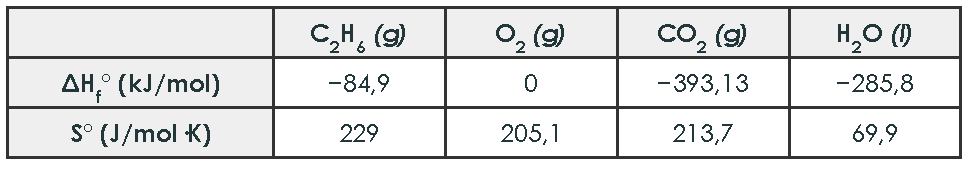
\includegraphics[width=0.75\linewidth]{FigurasSVG/UD4_Termodinamica/pdf/UD4_E03_tabla_EvAU_2013.pdf}
        %\caption{}
        %\label{fig:}
    \end{figure}

    \begin{enumerate}[label=\letraminuscula]
    \item Calcula la variación de entalpía y de entropía, en condiciones estándar, para la combustión del etano.
    \item Calcula \(\Delta G^0\) para la reacción anterior e indica si esta es espontánea a 298 K y 1 atm
    \end{enumerate}
    \begin{solu}

        La tabla adjunta proporciona los siguientes datos:

        \begin{center}
        \begin{tabular}{lcccc}
            \toprule
            & \ch{C2H6 \gas{}} & \ch{O2 \gas{}} & \ch{CO2 \gas{}} & \ch{H2O \lqd{}} \\
            \midrule
            \(\Delta H^0_f\) (kJ/mol) & \(-84,9\) & \(0\) & \(-393,13\) & \(-285,8\) \\
            \(S^0\) (J/mol·K) & \(229\) & \(205,1\) & \(213,7\) & \(69,9\) \\
            \bottomrule
        \end{tabular}
        \end{center}

        \textbf{a) Entalpía y entropía de la combustión del etano}

        La reacción de combustión del etano, ajustada, es:

        \begin{equation*}
            \ch{C2H6 \gas{} + 7/2 O2 \gas{} -> 2 CO2 \gas{} + 3 H2O \lqd{}}
        \end{equation*}

        \begin{equation*}
            \Delta H^0 = \left[ 2\, \Delta H^0_f (\ch{CO2}) + 3\, \Delta H^0_f (\ch{H2O}) \right] - \left[ \Delta H^0_f (\ch{C2H6}) + \dfrac{7}{2}\, \Delta H^0_f (\ch{O2}) \right]
        \end{equation*}

        \begin{equation*}
            \Delta H^0 = \left[ 2(-393,13) + 3(-285,8) \right] - \left[ -84,9 + 0 \right] = -1643,66 + 84,9 = \energia[kjmol]{-1558.76}
        \end{equation*}

        \begin{equation*}
            \Delta S^0 = \left[ 2\, S^0 (\ch{CO2}) + 3\, S^0 (\ch{H2O}) \right] - \left[ S^0 (\ch{C2H6}) + \dfrac{7}{2}\, S^0 (\ch{O2}) \right]
        \end{equation*}

        \begin{equation*}
            \Delta S^0 = \left[ 2(213,7) + 3(69,9) \right] - \left[ 229 + 3,5(205,1) \right] = 637,1 - 946,85 = \SI{-309.75}{\jpmolpk}
        \end{equation*}

        \textbf{b) Energía de Gibbs y espontaneidad}

        A \(T = \SI{298}{\kelvin}\):

        \begin{equation*}
            \Delta G^0 = \Delta H^0 - T \Delta S^0 = -1558,76 - 298 \cdot (-0,30975) = -1558,76 + 92,3 = \energia[kj]{-1466.5}
        \end{equation*}

        Como \(\Delta G^0 < 0\), la reacción \textbf{es espontánea} a 298 K y 1 atm.

    \end{solu}
\end{exerciseEVAU}

\begin{exerciseEVAU}
    \textbf{2013} Sabiendo que, a 298 K y 1 atm, las entalpías de combustión del hidrógeno, carbono y eteno son,
    respectivamente, \energia[kjmol]{-285,5},  \energia[kjmol]{-393,13} y \energia[kjmol]{-1421,2}, a) escribe las reacciones correspondientes a las combustiones citadas; b) calcula la entalpía de formación del eteno; c) calcula la energía que se desprenderá, en las condiciones de presión y temperatura anteriores, al obtener 40 L de \ch{CO2} mediante combustión del eteno.
    \datos{}: \(R = \ctegases\)

    \begin{solu}

        \textbf{a) Ecuaciones de combustión}

        Combustión del hidrógeno (formación del agua):

        \begin{equation*}
            \ch{H2 \gas{} + 1/2 O2 \gas{} -> H2O \lqd{}} \quad \Delta H^0_1 = \energia[kjmol]{-285.5}
        \end{equation*}

        Combustión del carbono (formación del \ch{CO2}):

        \begin{equation*}
            \ch{C \sld{} + O2 \gas{} -> CO2 \gas{}} \quad \Delta H^0_2 = \energia[kjmol]{-393.13}
        \end{equation*}

        Combustión del eteno:

        \begin{equation*}
            \ch{C2H4 \gas{} + 3 O2 \gas{} -> 2 CO2 \gas{} + 2 H2O \lqd{}} \quad \Delta H^0_3 = \energia[kjmol]{-1421.2}
        \end{equation*}

        \textbf{b) Entalpía de formación del eteno}

        La reacción de formación del eteno es \(\ch{2 C \sld{} + 2 H2 \gas{} -> C2H4 \gas{}}\). Por la ley de Hess:

        \begin{equation*}
            \Delta H^0_3 = \left[ 2\, \Delta H^0_2 + 2\, \Delta H^0_1 \right] - \Delta H^0_f (\ch{C2H4})
        \end{equation*}

        \begin{equation*}
            -1421,2 = \left[ 2(-393,13) + 2(-285,5) \right] - \Delta H^0_f (\ch{C2H4}) = -1357,26 - \Delta H^0_f (\ch{C2H4})
        \end{equation*}

        \begin{equation*}
            \Delta H^0_f (\ch{C2H4}) = -1357,26 + 1421,2 = \energia[kjmol]{63.9}
        \end{equation*}

        \textbf{c) Energía desprendida al obtener 40 L de \ch{CO2}}

        A \(T = \temperatura[k]{298}\) y \(P = \SI{1}{\atmospher}\):

        \begin{equation*}
            n(\ch{CO2}) = \dfrac{PV}{RT} = \dfrac{1 \times 40}{0,082 \times 298} = 1,637 \ \text{mol}
        \end{equation*}

        Como en la combustión del eteno se forman 2 mol de \ch{CO2} por cada mol de \ch{C2H4}, liberando \(1421,2\) kJ, la energía por mol de \ch{CO2} es:

        \begin{equation*}
            \dfrac{\Delta H^0_3}{2} = \dfrac{-1421,2}{2} = \energia[kjmol]{-710.6}
        \end{equation*}

        \begin{equation*}
            q = 1,637 \ \text{mol} \times \energia[kjmol]{710.6} = \energia[kj]{1163.5}
        \end{equation*}

    \end{solu}
\end{exerciseEVAU}

\begin{exerciseEVAU}
    \textbf{2013} Justifica el signo (positivo o negativo) de la variación de entropía y de entalpía de una reacción
    química sabiendo que esta se produce espontáneamente a temperaturas elevadas, pero que no lo hace a baja temperatura.

    \begin{solu}

        La espontaneidad de una reacción viene dada por el signo de \(\Delta G = \Delta H - T \Delta S\).

        Para que la reacción \textbf{no sea espontánea a baja temperatura} pero \textbf{sí lo sea a temperatura elevada}, el término \(-T \Delta S\) debe ser el que, al aumentar \(T\), termine dominando sobre \(\Delta H\) y haga que \(\Delta G\) pase de ser positivo a negativo.

        Esto solo es posible si:
        \begin{itemize}
            \item \(\boldsymbol{\Delta H > 0}\) (reacción endotérmica): a baja temperatura, \(\Delta H\) domina y \(\Delta G > 0\) (no espontánea).
            \item \(\boldsymbol{\Delta S > 0}\) (aumenta el desorden): así, al crecer \(T\), el término \(-T\Delta S\) se hace cada vez más negativo, hasta lograr que \(\Delta G = \Delta H - T\Delta S\) sea negativo (espontánea) a temperaturas suficientemente altas.
        \end{itemize}

        Si \(\Delta S\) fuera negativo, el término \(-T\Delta S\) sería siempre positivo y, sumado a un \(\Delta H>0\), la reacción nunca sería espontánea, independientemente de la temperatura; y si \(\Delta H\) fuera negativo, la reacción sería espontánea también a bajas temperaturas. Por tanto, la única combinación coherente con el enunciado es \(\Delta H > 0\) y \(\Delta S > 0\).

    \end{solu}
\end{exerciseEVAU}

\begin{exerciseEVAU}
    \textbf{2013} Sabiendo que las entalpías de combustión, en condiciones estándar, del monóxido de carbono
    (obteniéndose dióxido de carbono), del hidrógeno (obteniéndose agua líquida) y del metano son \energia[kjmol]{-283,0}, \energia[kjmol]{-285,8} y \energia[kjmol]{-890,3}: a) escribe las reacciones de combustión ajustadas; b) calcula \(\Delta H^0\) para la reacción siguiente: \ch{4 CO \gas{} + 8 H2 \gas{} -> 3 CH4 \gas{} + CO2 \gas{} + 2 H2O \lqd{}} ; c) calcula la energía desprendida en la obtención de 56 gramos de metano mediante la reacción anterior.
    \datos{}: Masas atómicas: C = 12; H = 1.

    \begin{solu}

        \textbf{a) Reacciones de combustión ajustadas}

        \begin{align*}
            \text{(1)} \quad & \ch{CO \gas{} + 1/2 O2 \gas{} -> CO2 \gas{}} \quad \Delta H^0_1 = \energia[kjmol]{-283.0} \\
            \text{(2)} \quad & \ch{H2 \gas{} + 1/2 O2 \gas{} -> H2O \lqd{}} \quad \Delta H^0_2 = \energia[kjmol]{-285.8} \\
            \text{(3)} \quad & \ch{CH4 \gas{} + 2 O2 \gas{} -> CO2 \gas{} + 2 H2O \lqd{}} \quad \Delta H^0_3 = \energia[kjmol]{-890.3}
        \end{align*}

        \textbf{b) \(\Delta H^0\) de la reacción} \(\ch{4 CO \gas{} + 8 H2 \gas{} -> 3 CH4 \gas{} + CO2 \gas{} + 2 H2O \lqd{}}\)

        Combinamos las reacciones anteriores mediante la ley de Hess: tomamos 4 veces la reacción (1), 8 veces la reacción (2) y restamos 3 veces la reacción (3) (para que el \ch{CH4} pase, invertido, al lado de los productos):

        \begin{equation*}
            \Delta H^0 = 4\, \Delta H^0_1 + 8\, \Delta H^0_2 - 3\, \Delta H^0_3
        \end{equation*}

        \begin{equation*}
            \Delta H^0 = 4(-283,0) + 8(-285,8) - 3(-890,3) = -1132,0 - 2286,4 + 2670,9 = \energia[kjmol]{-747.5}
        \end{equation*}

        Comprobación de la suma de ecuaciones: \(4\,\ch{CO} + 2\,\ch{O2} + 8\,\ch{H2} + 4\,\ch{O2} + 3\,\ch{CO2} + 6\,\ch{H2O} \to 4\,\ch{CO2} + 8\,\ch{H2O} + 3\,\ch{CH4} + 6\,\ch{O2}\), que al cancelar especies comunes a ambos lados (\(6\,\ch{O2}\), \(3\,\ch{CO2}\) y \(6\,\ch{H2O}\)) da exactamente la reacción del enunciado.

        \textbf{c) Energía desprendida al obtener 56 g de metano}

        La masa molar del metano es \(M(\ch{CH4}) = 12 + 4(1) = \SI{16}{\gram\per\mole}\), por lo que:

        \begin{equation*}
            n(\ch{CH4}) = \dfrac{56 \ \si{\gram}}{16 \ \si{\gram\per\mole}} = 3,5 \ \text{mol}
        \end{equation*}

        Como la reacción, tal y como está ajustada, produce 3 mol de \ch{CH4} liberando \(747,5\) kJ, la energía liberada por mol de \ch{CH4} formado es \(747,5/3 = \energia[kjmol]{249.2}\), y para 3,5 mol:

        \begin{equation*}
            q = 3,5 \ \text{mol} \times \energia[kjmol]{249.2} = \energia[kj]{872.1}
        \end{equation*}

    \end{solu}
\end{exerciseEVAU}

\begin{exerciseEVAU}
    \textbf{2013} El hierro se obtiene en los altos hornos mediante la reacción siguiente, cuya variación de entalpía
    estándar es \energia[kjmol]{-24,77} de \ch{Fe2O3}: \ch{Fe2O3 \sld{} + 3 CO \gas{} -> 2 Fe \sld{} + 3 CO2 \gas{}} . Calcula: a) la energía desprendida en la obtención de 1 tonelada de hierro; b) la entalpía estándar de formación del monóxido de carbono, sabiendo que las entalpías estándar de formación del \ch{Fe2O3 \sld{}} y del \ch{CO2 \gas{}} son \energia[kjmol]{-824,2} y \energia[kjmol]{-393,51}, respectivamente. c) Si \(\Delta S^0\) de la reacción de obtención del hierro es \SI{14,63}{\joule\per\mole\per\kelvin}, indica razonadamente si dicha reacción es espontánea a cualquier temperatura. (\datos{}: Masas atómicas: Fe = 55,85 ; O = 16).

    \begin{solu}

        \textbf{a) Energía desprendida en la obtención de 1 tonelada de hierro}

        Los moles de hierro contenidos en 1 tonelada (\(10^6\) g) son:

        \begin{equation*}
            n(\ch{Fe}) = \dfrac{10^6 \ \si{\gram}}{55,85 \ \si{\gram\per\mole}} = 17\,904,7 \ \text{mol}
        \end{equation*}

        Como la reacción, tal como está ajustada, produce 2 mol de \ch{Fe} por cada mol de \ch{Fe2O3} que reacciona, liberando \(24,77\) kJ, la energía por mol de \ch{Fe} formado es \(24,77/2 = \energia[kjmol]{12.385}\):

        \begin{equation*}
            q = 17\,904,7 \ \text{mol} \times \energia[kjmol]{12.385} \approx \energia[kj]{221821}
        \end{equation*}

        \textbf{b) Entalpía estándar de formación del monóxido de carbono}

        Aplicando la ley de Hess a la reacción de obtención del hierro:

        \begin{equation*}
            \Delta H^0 = \left[ 2\, \Delta H^0_f (\ch{Fe}) + 3\, \Delta H^0_f (\ch{CO2}) \right] - \left[ \Delta H^0_f (\ch{Fe2O3}) + 3\, \Delta H^0_f (\ch{CO}) \right]
        \end{equation*}

        \begin{equation*}
            -24,77 = \left[ 0 + 3(-393,51) \right] - \left[ -824,2 + 3\, \Delta H^0_f (\ch{CO}) \right]
        \end{equation*}

        \begin{equation*}
            -24,77 = -1180,53 + 824,2 - 3\, \Delta H^0_f (\ch{CO}) = -356,33 - 3\, \Delta H^0_f (\ch{CO})
        \end{equation*}

        \begin{equation*}
            \Delta H^0_f (\ch{CO}) = \dfrac{-356,33 + 24,77}{-3} = \dfrac{-331,56}{-3} = \energia[kjmol]{-110.5}
        \end{equation*}

        \textbf{c) Espontaneidad a cualquier temperatura}

        Tenemos \(\Delta H^0 = \energia[kjmol]{-24.77} < 0\) (exotérmica) y \(\Delta S^0 = \SI{14.63}{\jpmolpk} > 0\) (aumenta el desorden, coherente con que se forman 3 mol de gas \ch{CO2} a partir de 3 mol de gas \ch{CO} más un sólido, sin apenas variación neta del número de moles gaseosos, aunque sí de la naturaleza de las especies).

        Como en \(\Delta G^0 = \Delta H^0 - T \Delta S^0\) el primer término es negativo y el segundo término, \(-T\Delta S^0\), también es negativo para cualquier \(T>0\) (ya que \(\Delta S^0>0\)), se cumple que \(\Delta G^0 < 0\) para \textbf{cualquier temperatura}. Por tanto, la reacción de obtención de hierro en el alto horno es espontánea a cualquier temperatura.

    \end{solu}
\end{exerciseEVAU}

\begin{exerciseEVAU}
    \textbf{2012} Sea la reacción química \ch{F2 \gas{} + 2 HCl \gas{} -> 2 HF \gas{} + Cl2 \gas{}}, cuya variación de entropía estándar vale \SI{-6,04}{\joule\per\mole\per\kelvin}. Se sabe que en la reacción de 2 litros de \ch{F2 \gas{}} en condiciones estándar se desprenden \energia[kj]{28,87}. Calcula:
    \begin{enumerate}[label=\letraminuscula]
    \item \(\Delta H^0\) de la reacción.
    \item \(\Delta G^0\) de la reacción.
    \item ¿Será espontánea la reacción a \temperatura[c]{300}? Justifica tu respuesta.
    \end{enumerate}
    (\datos{}:  \(R = \ctegases\))

    \begin{solu}

        \textbf{a) \(\Delta H^0\) de la reacción}

        En condiciones estándar (\(T = \temperatura[k]{298}\), \(P = \SI{1}{\atmospher}\)), los moles de \ch{F2} contenidos en 2 L son:

        \begin{equation*}
            n(\ch{F2}) = \dfrac{PV}{RT} = \dfrac{1 \times 2}{0,082 \times 298} = 0,0819 \ \text{mol}
        \end{equation*}

        Como la reacción, tal como está ajustada, consume 1 mol de \ch{F2} y en la reacción de esos 0,0819 mol se desprenden 28,87 kJ:

        \begin{equation*}
            \Delta H^0 = \dfrac{-28,87 \ \si{\kilo\joule}}{0,0819 \ \text{mol}} = \energia[kjmol]{-352.7}
        \end{equation*}

        \textbf{b) \(\Delta G^0\) de la reacción}

        \begin{equation*}
            \Delta G^0 = \Delta H^0 - T \Delta S^0 = -352,7 - 298 \cdot (-0,00604) = -352,7 + 1,8 = \energia[kjmol]{-350.9}
        \end{equation*}

        \textbf{c) Espontaneidad a \SI{300}{\celsius}}

        A \(T = \SI{573}{\kelvin}\):

        \begin{equation*}
            \Delta G^0_{573} = \Delta H^0 - T \Delta S^0 = -352,7 - 573 \cdot (-0,00604) = -352,7 + 3,46 = \energia[kjmol]{-349.2}
        \end{equation*}

        Como \(\Delta G^0_{573} < 0\), la reacción \textbf{sigue siendo espontánea} a \SI{300}{\celsius}. De hecho, dado que \(|\Delta H^0|\) es muy grande frente al término \(T\Delta S^0\) (que apenas varía con la temperatura, ya que \(\Delta S^0\) es pequeño), esta reacción es espontánea prácticamente a cualquier temperatura.

    \end{solu}
\end{exerciseEVAU}

\begin{exerciseEVAU}
    \textbf{2012} La entalpía estándar de combustión del propano es \energia[kjmol]{-2200} y las entalpías estándar de formación del agua en estado líquido y del dióxido de carbono son, respectivamente, \energia[kjmol]{-285,5} y \energia[kjmol]{-393}. Calcula: a) los kg de antracita que se deben quemar para producir la misma cantidad de energía que la obtenida en la combustión de 100 g de propano, sabiendo que al quemar 1 g de antracita se desprenden \energia[kj]{34,3}; b) la entalpía estándar de formación del propano; c) el volumen de dióxido de carbono obtenido en la combustión de 100 gramos
    de propano en condiciones estándar. (\datos{}: \(R = \ctegases\); masas atómicas: C = 12; O = 16; H = 1).

    \begin{solu}

        \textbf{a) Kg de antracita equivalentes a 100 g de propano}

        La masa molar del propano es \(M(\ch{C3H8}) = 3(12) + 8(1) = \SI{44}{\gram\per\mole}\), por lo que:

        \begin{equation*}
            n(\ch{C3H8}) = \dfrac{100 \ \si{\gram}}{44 \ \si{\gram\per\mole}} = 2,273 \ \text{mol}
        \end{equation*}

        La energía liberada al quemar esos 100 g de propano es:

        \begin{equation*}
            q = 2,273 \ \text{mol} \times \energia[kjmol]{2200} = \energia[kj]{5000}
        \end{equation*}

        Como cada gramo de antracita libera 34,3 kJ, la masa de antracita necesaria para obtener esos 5000 kJ es:

        \begin{equation*}
            m = \dfrac{5000 \ \si{\kilo\joule}}{34,3 \ \si{\kilo\joule\per\gram}} = 145,8 \ \si{\gram} = \SI{0.1458}{\kilo\gram}
        \end{equation*}

        \textbf{b) Entalpía estándar de formación del propano}

        La reacción de combustión es \(\ch{C3H8 \gas{} + 5 O2 \gas{} -> 3 CO2 \gas{} + 4 H2O \lqd{}}\). Por la ley de Hess:

        \begin{equation*}
            \Delta H^0_{comb} = \left[ 3\, \Delta H^0_f (\ch{CO2}) + 4\, \Delta H^0_f (\ch{H2O}) \right] - \Delta H^0_f (\ch{C3H8})
        \end{equation*}

        \begin{equation*}
            -2200 = \left[ 3(-393) + 4(-285,5) \right] - \Delta H^0_f (\ch{C3H8}) = -2321 - \Delta H^0_f (\ch{C3H8})
        \end{equation*}

        \begin{equation*}
            \Delta H^0_f (\ch{C3H8}) = -2321 + 2200 = \energia[kjmol]{-121}
        \end{equation*}

        \textbf{c) Volumen de \ch{CO2} obtenido en la combustión de 100 g de propano}

        Como cada mol de propano produce 3 mol de \ch{CO2}:

        \begin{equation*}
            n(\ch{CO2}) = 3 \times 2,273 = 6,818 \ \text{mol}
        \end{equation*}

        En condiciones estándar (\(T = \temperatura[k]{298}\), \(P = \SI{1}{\atmospher}\)):

        \begin{equation*}
            V = \dfrac{nRT}{P} = \dfrac{6,818 \times 0,082 \times 298}{1} = 166,6 \ \si{\litre}
        \end{equation*}

    \end{solu}
\end{exerciseEVAU}

\begin{exerciseEVAU}
    \textbf{2012} Una reacción es espontánea a altas temperaturas y no lo es a bajas temperaturas. Justifica los signos, positivos o negativos, de los valores de su variación de entalpía, \(\Delta H\), y de su variación de entropía, \(\Delta S\).

    \begin{solu}

        Al igual que en el razonamiento anterior, la espontaneidad depende del signo de \(\Delta G = \Delta H - T \Delta S\).

        Para que la reacción \textbf{no sea espontánea a baja temperatura} (\(\Delta G > 0\)) pero \textbf{sí lo sea a temperatura elevada} (\(\Delta G < 0\)), es necesario que:

        \begin{itemize}
            \item \(\boldsymbol{\Delta H > 0}\) (reacción endotérmica), de forma que a baja temperatura, donde el término \(-T\Delta S\) es pequeño, predomine \(\Delta H\) y \(\Delta G\) resulte positivo.
            \item \(\boldsymbol{\Delta S > 0}\) (aumenta el desorden del sistema), de forma que al aumentar la temperatura el término \(-T\Delta S\) se haga cada vez más negativo, hasta compensar y superar a \(\Delta H\), logrando \(\Delta G < 0\).
        \end{itemize}

    \end{solu}
\end{exerciseEVAU}

\begin{exerciseEVAU}
    \textbf{2012} La variación de entalpía estándar de la reacción de combustión del etano es \energia[kjmol]{-1559,8}, considerando que el agua queda en estado líquido. Sabiendo que las entalpías de formación del agua líquida y del dióxido de carbono gaseoso son \energia[kjmol]{-285,8}  y \energia[kjmol]{-393,5}, respectivamente, calcula: a) \(\Delta H^0\) de la reacción de formación del etano; b) la energía desprendida en la combustión de 3 litros de etano medidos a 300 K y 2 atm; c) los gramos de agua que se obtienen en la reacción anterior.
    (\datos{}: \(R = \ctegases\); masas atómicas: H = 1 ; O = 16)

    \begin{solu}

        \textbf{a) \(\Delta H^0\) de formación del etano}

        La reacción de combustión es \(\ch{C2H6 \gas{} + 7/2 O2 \gas{} -> 2 CO2 \gas{} + 3 H2O \lqd{}}\). Por la ley de Hess:

        \begin{equation*}
            \Delta H^0_{comb} = \left[ 2\, \Delta H^0_f (\ch{CO2}) + 3\, \Delta H^0_f (\ch{H2O}) \right] - \Delta H^0_f (\ch{C2H6})
        \end{equation*}

        \begin{equation*}
            -1559,8 = \left[ 2(-393,5) + 3(-285,8) \right] - \Delta H^0_f (\ch{C2H6}) = -1644,4 - \Delta H^0_f (\ch{C2H6})
        \end{equation*}

        \begin{equation*}
            \Delta H^0_f (\ch{C2H6}) = -1644,4 + 1559,8 = \energia[kjmol]{-84.6}
        \end{equation*}

        \textbf{b) Energía desprendida en la combustión de 3 L de etano a 300 K y 2 atm}

        \begin{equation*}
            n(\ch{C2H6}) = \dfrac{PV}{RT} = \dfrac{2 \times 3}{0,082 \times 300} = 0,2439 \ \text{mol}
        \end{equation*}

        \begin{equation*}
            q = 0,2439 \ \text{mol} \times \energia[kjmol]{1559.8} = \energia[kj]{380.5}
        \end{equation*}

        \textbf{c) Gramos de agua obtenidos}

        Como se forman 3 mol de \ch{H2O} por cada mol de etano quemado:

        \begin{equation*}
            n(\ch{H2O}) = 3 \times 0,2439 = 0,7317 \ \text{mol}
        \end{equation*}

        \begin{equation*}
            m(\ch{H2O}) = 0,7317 \ \text{mol} \times 18 \ \si{\gram\per\mole} = \SI{13.2}{\gram}
        \end{equation*}

    \end{solu}
\end{exerciseEVAU}

\begin{exerciseEVAU}
    \textbf{2012} Justifica el signo (\(+\) o \(-\)) de la variación de entalpía y de energía libre de Gibbs del siguiente proceso a
    temperatura y presión ambiente: “un cohete pirotécnico que explota únicamente cuando se enciende la mecha”.

    \begin{solu}

        \textbf{Signo de \(\Delta H\)}

        La explosión de un cohete pirotécnico libera luz y una gran cantidad de calor de forma súbita, por lo que se trata de un proceso claramente exotérmico: \(\boldsymbol{\Delta H < 0}\).

        \textbf{Signo de \(\Delta G\)}

        En la explosión, el material sólido (o líquido) de la carga pirotécnica se transforma en una gran cantidad de gases a alta temperatura, lo que supone un enorme aumento del desorden del sistema (\(\Delta S \gg 0\)). Junto con \(\Delta H < 0\), esto hace que \(\Delta G = \Delta H - T \Delta S\) sea muy negativo: \(\boldsymbol{\Delta G < 0}\), es decir, el proceso es termodinámicamente muy favorable (espontáneo) una vez que se inicia.

        \textbf{¿Por qué necesita entonces la mecha?}

        Aunque el proceso es termodinámicamente espontáneo (\(\Delta G < 0\)), esto no implica que ocurra por sí solo a temperatura ambiente: la reacción tiene una elevada energía de activación (barrera cinética) que impide que se inicie de manera espontánea. La mecha aporta la energía necesaria para superar esa barrera y desencadenar la reacción, que después se automantiene y acelera gracias al enorme calor liberado (exotermicidad). Esto ilustra que la espontaneidad termodinámica (\(\Delta G\)) y la velocidad de una reacción (cinética) son cuestiones independientes.

    \end{solu}
\end{exerciseEVAU}

\begin{exerciseEVAU}
    \textbf{2012}. La gasolina puede ser considerada como una mezcla de hidrocarburos de ocho átomos de carbono, de
    fórmula \ch{C8H18}. Sabiendo que las entalpías estándar de formación del agua líquida, del dióxido de carbono y de la
    gasolina son \energia[kjmol]{-285,5}, \energia[kjmol]{-393} y \energia[kjmol]{-268,8}, respectivamente, calcula:
    a) La entalpía estándar de combustión de la gasolina. b) La energía desprendida en la combustión de 5 litros de gasolina, sabiendo que su densidad es \SI{800}{\kilo\g\per\cubic\metre}. c) El volumen de dióxido de carbono medido en condiciones estándar que se producirá en dicha combustión.
    (\datos{}: \(R = \ctegases{}\); masas atómicas: C = 12 ; H = 1)

    \begin{solu}

        \textbf{a) Entalpía estándar de combustión de la gasolina}

        La reacción de combustión ajustada del octano es:

        \begin{equation*}
            \ch{C8H18 \lqd{} + 25/2 O2 \gas{} -> 8 CO2 \gas{} + 9 H2O \lqd{}}
        \end{equation*}

        Por la ley de Hess:

        \begin{equation*}
            \Delta H^0_{comb} = \left[ 8\, \Delta H^0_f (\ch{CO2}) + 9\, \Delta H^0_f (\ch{H2O}) \right] - \Delta H^0_f (\ch{C8H18})
        \end{equation*}

        \begin{equation*}
            \Delta H^0_{comb} = \left[ 8(-393) + 9(-285,5) \right] - (-268,8) = -5713,5 + 268,8 = \energia[kjmol]{-5444.7}
        \end{equation*}

        \textbf{b) Energía desprendida en la combustión de 5 L de gasolina}

        Con una densidad de \(\SI{800}{\kilo\g\per\cubic\metre} = \SI{0.8}{\kilo\g\per\litre}\), la masa de 5 L de gasolina es:

        \begin{equation*}
            m = 5 \ \si{\litre} \times 0,8 \ \si{\kilo\g\per\litre} = \SI{4}{\kilo\gram} = \SI{4000}{\gram}
        \end{equation*}

        La masa molar de la gasolina (\ch{C8H18}) es \(M = 8(12) + 18(1) = \SI{114}{\gram\per\mole}\), por lo que:

        \begin{equation*}
            n = \dfrac{4000 \ \si{\gram}}{114 \ \si{\gram\per\mole}} = 35,09 \ \text{mol}
        \end{equation*}

        \begin{equation*}
            q = 35,09 \ \text{mol} \times \energia[kjmol]{5444.7} \approx \energia[kj]{191041}
        \end{equation*}

        \textbf{c) Volumen de \ch{CO2} obtenido}

        Como por cada mol de gasolina se forman 8 mol de \ch{CO2}:

        \begin{equation*}
            n(\ch{CO2}) = 8 \times 35,09 = 280,7 \ \text{mol}
        \end{equation*}

        En condiciones estándar (\(T = \temperatura[k]{298}\), \(P = \SI{1}{\atmospher}\)):

        \begin{equation*}
            V = \dfrac{nRT}{P} = \dfrac{280,7 \times 0,082 \times 298}{1} \approx \SI{6859}{\litre} \approx \SI{6.86}{\cubic\metre}
        \end{equation*}

    \end{solu}
\end{exerciseEVAU}

\newpage

\begin{figure}[H]
    \centering
    % [FIGURA ORIGINAL] \includegraphics[scale=1]{images/imagesUD4Termidonamica/UD4_Problemas/entalpias_de_formacion_estandar.png}
    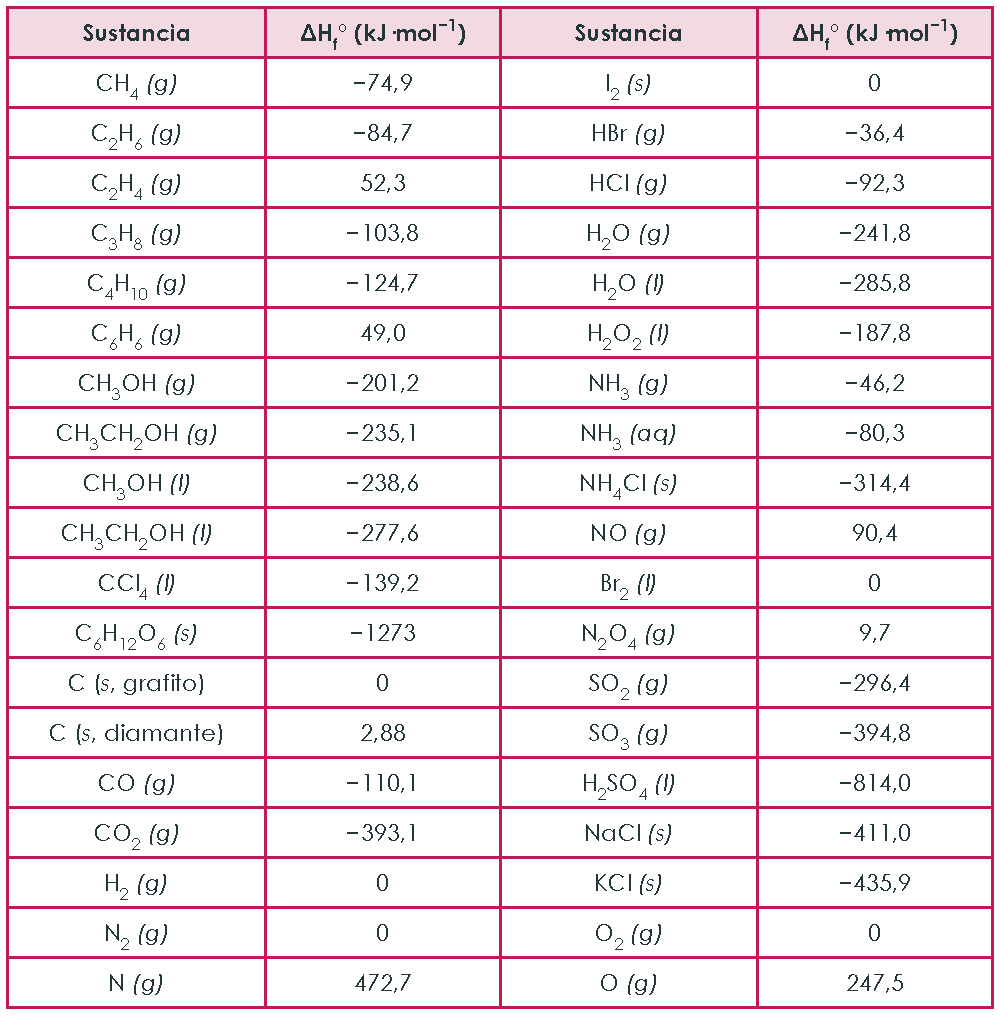
\includegraphics[width=0.8\linewidth]{FigurasSVG/UD4_Termodinamica/pdf/UD4_E04_entalpias_formacion.pdf}
    \caption{Entalpías de formación}
    \label{fig:entalpias_de_formacion}
\end{figure}

\begin{figure}[H]
    \centering
    % [FIGURA ORIGINAL] \includegraphics[scale=.5]{images/imagesUD4Termidonamica/UD4_Problemas/entalpias_de_enlace.png}
    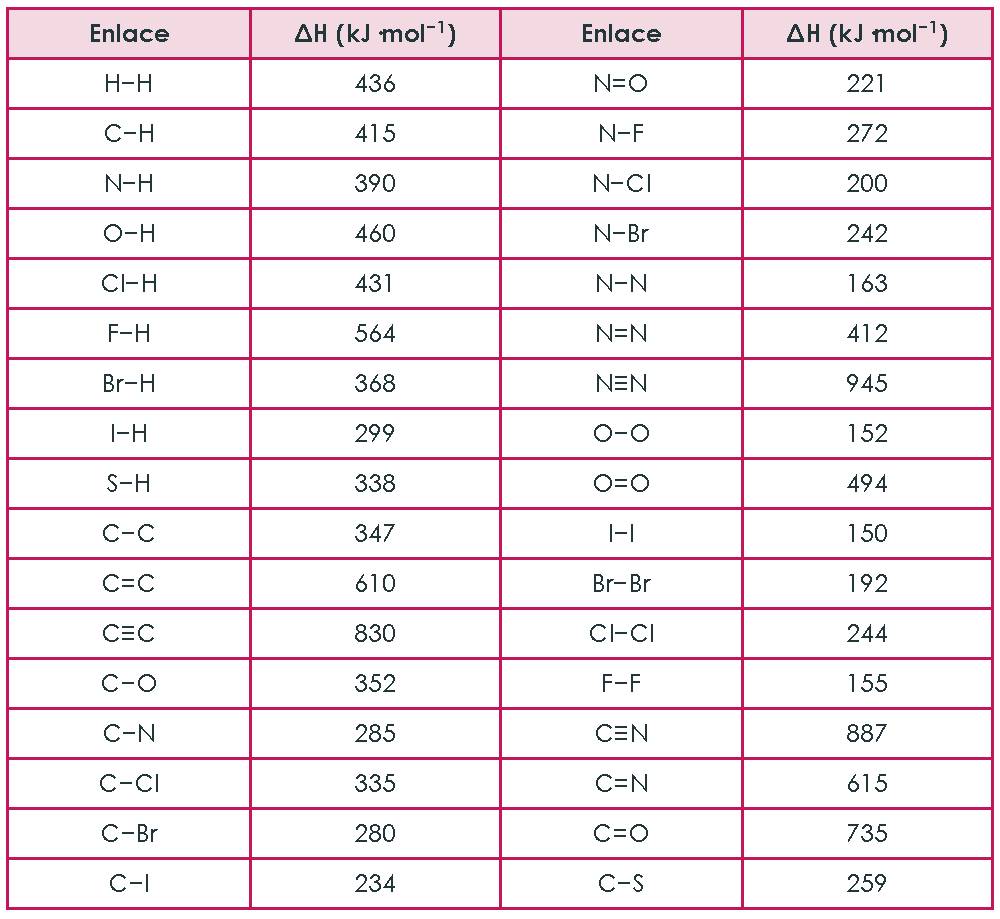
\includegraphics[width=0.75\linewidth]{FigurasSVG/UD4_Termodinamica/pdf/UD4_E05_entalpias_enlace.pdf}
    \caption{Entalpías de enlace}
    \label{fig:entalpias_de_enlace}
\end{figure}

